

% !TeX root = RJwrapper.tex
\title{bootCT: An R Package for Bootstrap Cointegration Tests in ARDL Models}
\author{by Gianmarco Vacca, Maria Zoia, Stefano Bertelli}

\maketitle
\nocite{RSOFT}
\abstract{
The Autoregressive Distributed Lag approach to cointegration or bound testing, proposed by Pesaran in 2001, has become prominent in empirical research. Although this approach has many advantages over the classical cointegration tests, it is not exempt from drawbacks, such as  possible inconclusive inference and distortion in size.
Recently, Bertelli and coauthors developed a bootstrap approach to the bound tests to overcome these drawbacks. This paper introduces the R package bootCT, which implements this method by deriving the bootstrap versions of the bound tests and of the asymptotic F-test on the independent variables proposed by Sam and coauthors in 2019.
As a spinoff, a general method for generating random multivariate time series following a given VECM/ARDL structure is provided in the package. 
Empirical applications showcase the main functionality of the package.
}

\section{Introduction}\label{sec:intro}
 Cointegration and error correction are fundamental concepts in the analysis of economic data, insofar as they provide an appropriate framework for testing economic hypotheses about growth and fluctuation. 
 Several approaches have been proposed in the literature to determine whether two or more non-stationary time series are cointegrated, meaning they share a common long-run relationship.\\ 
There are two basic types of tests for cointegration: single equation tests and VAR-based tests. The former check the presence of unit roots in cointegration residuals \citep[see, e.g.,][]{engle1987co,engleyoo87,Mackinnon91,gabriel2002,cook2006power} or test the significance of the error-correction (EC) term coefficient \citep{kremers1992power,maddala1998,arranz2000,ericsson2002}. The latter, such as the \citet{johansen1991} approach, tackle the problem of detecting cointegrating relationships in a VAR model.
This latter approach, albeit having the advantage of avoiding the issue of normalization, as well as allowing the detection of multiple cointegrating vectors, is far from being perfect. In the VAR system all variables are treated symmetrically, as opposed to the standard univariate models that usually have a clear interpretation in terms of exogenous and endogenous variables. Furthermore, in a VAR system all the variables are estimated at the same time, which is problematic if the relation between some variables is flawed, that is affected by some source of error. In this case a simultaneous estimation process tends to propagate the error affecting one equation to the others.   
Furthermore, a multidimensional VAR models employs plenty of degrees of freedom.\\
The recent cointegration approach, known as Autoregressive Distributed Lag (ARDL) approach to cointegration or bound testing, proposed by ~\citet{pesaran2001} (PSS), falls in the former strand of literature. It has become prominent in empirical research because it shows several advantages with respect to traditional methods for testing cointegration. First, it is applicable also in cases of mixed order integrated variables, albeit with integration not exceeding the first order.   
Thus, it evades the necessity of pre-testing the variables and, accordingly, avoids some common practices that may prevent finding cointegrating relationships, such as dropping variables or transforming them into stationary form ~\citep[see][]{mcnown2018bootstrapping}.
Second, cointegration bound tests are performed in an ARDL model that allows different lag orders for each variable, thus providing a more flexible framework than other commonly employed approaches.
Finally, unlike other cointegration techniques, which are sensitive to the sample size, the ARDL approach provides robust and consistent results for small sample sizes.\\ 
Notably, the ARDL bound testing methodology has quickly spread in economics and econometrics to study the cointegrating relationships between macroeconomic and financial variables, to evaluate the long-run impact of energy variables, or to assess recent environmental policies and their impact on the economy. Among the many applications, see for instance \citet{haseeb2019impact,reda2020using, menegaki2019ardl,yilanci2020brics,hussain2019environmental,abbasi2021energy}.\\
The original bound tests proposed by \citet{pesaran2001} are an $F$-test for the significance of the coefficients of all lagged level variables entering the error correction term ($F_{ov}$), and a $t$-test for the coefficient of the lagged dependent variable. When either the dependent or the independent variables do not appear in the long-run relationship, a degenerate case arises. The bound $t$-test provides answers on the occurrence of a degenerate case of second type, while the occurrence of a degeneracy case of first type can be assessed by testing whether the dependent variable is of integration order I(1).
This type of check violates the spirit and motivation of the bound tests, which are supposed to be applicable in situations of unknown order of integration for the variables.\\ 
Recently, \citet{mcnown2018bootstrapping} pointed out how, due to the low power problem of unit root tests, investigating the presence of a first type degeneracy by testing the integration order of the dependent variable may lead to incorrect conclusions. Therefore, they suggested checking for its occurrence by testing the significance of the lagged levels of the independent variables via an extra $F$-test ($F_{ind}$), which was also worked out in its asymptotic version \citep[SMK;][]{sam2019augmented}.\\
Besides problems in testing the occurrence of degenerate cases, in general, the main drawback of the bound tests is the occurrence of potentially inconclusive results, if the test statistic lies between the bounds of the test distribution under the null. Furthermore, the asymptotic distributions of the statistics may provide a poor approximation of the true distributions in small samples. Finite sample critical values, even if only for a subset of all possible model specifications, have been worked out in the literature \citep[see][]{mills2001real,narayan2004crime,kanioura2005critical,narayan2005saving}, while \cite{kripfganz2020response} provided the quantiles of the asymptotic distributions of the tests as functions of the sample size, the lag order and the number of long-run forcing variables. However, this relevant improvement does not eliminate the uncertainty related to the inconclusive regions, or the existence of other critical issues related to the underlying assumptions of the bound test framework, such as the (weak) exogeneity of the independent variables or the non-stationarity of the dependent variable.\\
To overcome the mentioned bound test drawbacks, \cite{bertelli2022bootstrap} proposed bootstrapping the ARDL cointegration test. Inference can always be pursued with ARDL bootstrap tests, unlike what happens with both the PSS tests and the SMK test on the independent variables.
Bootstrap ARDL tests were first put forward by \cite{mcnown2018bootstrapping} in an unconditional ARDL model, which omits the instantaneous differences of the exogenous variables in the ARDL equation, rather than a conditional one, as originally proposed by \cite{pesaran2001}.
The unconditional model is often used, for reason of practical convenience, in empirical research. Simulation results in \cite{bertelli2022bootstrap} have highlighted the importance of employing the appropriate specification, especially under degenerate cases. In fact, it has been pointed out that a correct detection of these cases requires the comparison of the test outcomes in both the conditional and unconditional settings. Erroneous conclusions, based exclusively on one model specification, can thus be avoided.\\
In this paper, bootstrap bound tests, thereby including the bootstrap versions of the $F_{ov}$, $t$ and $F_{ind}$ bound tests, are carried out in a conditional ARDL model setting. This approach allows to overcome the problem of inconclusive regions of the standard bound tests. A comparison with the outcomes engendered by the unconditional ARDL bootstrap tests is nevertheless provided for the $F_{ind}$ test, to avoid erroneous inference in presence of degenerate cases.\\
The paper is organized as follows. Section \ref{sec:cointegration} introduces the theoretical results of the ARDL cointegration bound tests. Section \ref{sec:boot} details the steps carried out by the bootstrap procedure, which allows the construction of the (bootstrap) distribution - under the null - for the $F_{ov}$, $t$, conditional $F_{ind}$ and unconditional $F_{ind}$ tests. Section \ref{sec:pkg} introduces the \code{R} package \CRANpkg{bootCT} \citep{bootCT} and its functionalities: a method for the generation of random multivariate time series that follow a user-specified VECM/ARDL structure, with some examples, and the main function that carries out the aforementioned bootstrap tests, while also computing the PSS and SMK bound tests. 
The trade-off between accuracy and computational time of the bootstrap procedure is also investigated, under several scenarios in terms of sample size and number of replications. Notably, a function that performs the PSS bound tests is already available in the \CRANpkg{dynamac} package \citep{PKGDYNAMAC}, while no \code{R} routine has so far been implemented for the SMK test, to the best of our knowledge.
Section \ref{sec:app} gives some empirical applications that employ the core function of the package and its possible outputs. Section \ref{sec:end} concludes. Appendix \ref{sec:appendix} briefly delves into technical details of the conditional ARDL model and its possible specifications
\footnote{The \code{R} packages, either used in the creation of \CRANpkg{bootCT} or employed in the analyses presented in this paper, are \CRANpkg{magrittr} \citep{magrittr}, \CRANpkg{gtools} \citep{gtools}, \CRANpkg{pracma} \citep{pracma}, \CRANpkg{Rcpp} \citep{RCPP}, \CRANpkg{RcppArmadillo} \citep{RcppArmadillo2023}, \CRANpkg{Rmisc} \citep{Rmisc}, \CRANpkg{dynamac} \citep{PKGDYNAMAC}, \CRANpkg{ARDL} \citep{PKGARDL}, \CRANpkg{aod} \citep{aod}, \CRANpkg{vars} and \CRANpkg{urca} \citep{PKGVARS, urca}, \CRANpkg{aTSA} \citep{PKGATSA}, \CRANpkg{tseries} \citep{tseries}, \CRANpkg{reshape2},  \CRANpkg{ggplot2} and \CRANpkg{stringr} \citep{reshape2,ggplot,stringr}, \CRANpkg{tidyverse} and \CRANpkg{dplyr} \citep{tidyverse,dplyr}.}.

\section{Cointegration bound tests in ARDL models}\label{sec:cointegration}
The starting point of the approach proposed by ~\cite{pesaran2001} is a $(K+1)$ VAR($p$) model
\begin{equation}\label{eq:var}
\mathbf{A}(L)(\mathbf{z}_t-\boldsymbol{\mu}-\boldsymbol{\eta}t)=\boldsymbol{\varepsilon}_t \enspace \enspace \enspace \boldsymbol{\varepsilon}_t\sim N(\mathbf{0}, \boldsymbol{\Sigma}),\qquad\mathbf{A}(L)=\left(\mathbf{I}_{K+1}-  \sum_{j=1}^{p}\mathbf{A}_j\mathbf{L}^j\right)
\enspace \enspace \enspace t=1,2,\dots,T.
\end{equation}
Here, $\mathbf{A}_j$ are square $(K+1)$ matrices, $\mathbf{z}_t$ a vector of  $(K+1)$ variables, 
$\boldsymbol{\mu}$ and $\boldsymbol{\eta}$ are $(K+1)$ vectors representing the drift and the trend respectively, and $\det(\mathbf{A}(z))=0$ for $|z| \geq 1$. If the matrix $\mathbf{A}(1)=\mathbf{I}_{K+1}-\sum_{j=1}^{p}\mathbf{A}_{j}$ is singular, the components of $\mathbf{z}_t$ turn out to be integrated and possibly cointegrated.\\
The VECM representation of \eqref{eq:var} is given by (see Appendix \ref{sec:appendixa} for details)
\begin{equation}\label{eq:vecm}
\Delta\mathbf{z}_t=\boldsymbol{\alpha}_{0}+\boldsymbol{\alpha}_{1}t-\mathbf{A}(1)\mathbf{z}_{t-1}+\sum_{j=1}^{p-1}\boldsymbol{\Gamma}_{j}\Delta \mathbf{z}_{t-j}+\boldsymbol{\varepsilon}_t.
\end{equation}
Now, to study the adjustment to the equilibrium of a single variable $y_t$, given the other $\mathbf{x}_t$ variables, the vectors $\mathbf{z}_t$ and $\boldsymbol{\varepsilon}_t$ are partitioned
\begin{equation}\label{eq:vecpart}
\mathbf{z}_t=\begin{bmatrix}
\underset{(1,1)}{y_{t}}  \\ \underset{(K,1)}{\mathbf{x}_{t}}  
\end{bmatrix}, \enspace \enspace \enspace \boldsymbol{\varepsilon}_t=\begin{bmatrix}
\underset{(1,1)}{\varepsilon_{yt}} \\  \underset{(K,1)}{\boldsymbol{\varepsilon}_{xt}} 
\end{bmatrix}.
\end{equation}
%Furthermore, let us assume that 
 The matrix $\mathbf{A}(1)$, which is assumed to be singular to allow cointegration, is partitioned conformably to $\mathbf{z}_{t}$ as \footnote{ If the explanatory variables are stationary $\mathbf{A}_{xx}$ is non-singular ($rk(\mathbf{A}_{xx})=K$), while when they are integrated but without cointegrating relationship $\mathbf{A}_{xx}$ is a null matrix.} \\
\begin{equation}
   \mathbf{A}(1)=\begin{bmatrix}
\underset{(1,1)}{a_{yy}} & \underset{(1,K)}{\mathbf{a}_{yx}'} \\ \underset{(K,1)}{\mathbf{a}_{xy}} & \underset{(K,K)}{\mathbf{A}_{xx}}  
\end{bmatrix}.
\end{equation}
Under the assumption 
\begin{equation}\label{eq:normerr}
\boldsymbol{\varepsilon}_t \sim N\Bigg(\mathbf{0}, \begin{bmatrix}
\underset{(1,1)}{\sigma_{yy}}& \underset{(1,K)}{\boldsymbol{\sigma}_{yx}'}   \\ \underset{(K,1)}{\boldsymbol{\sigma}_{xy}} & \underset{(K,K)}{\boldsymbol{\Sigma}_{xx}} \end{bmatrix}\Bigg), 
\end{equation}
the following holds
\begin{equation}\label{eq:epsilonx}
\varepsilon_{yt}=\boldsymbol{\omega}'\boldsymbol{\varepsilon}_{xt}+\nu_{yt} \sim N(0,\sigma_{y.x}),      
\end{equation}
where $\sigma_{y.x}=\sigma_{yy}-\boldsymbol{\omega}'\boldsymbol{\sigma}_{xy}$ with $\boldsymbol{\omega}'=\boldsymbol{\sigma}'_{yx}\boldsymbol{\Sigma}^{-1}_{xx}$, and $\nu_{yt}$ is independent of $\boldsymbol{\varepsilon}_{xt}$.\\
Substituting \eqref{eq:epsilonx} into \eqref{eq:vecm} and assuming that the $\mathbf{x}_{t}$ variables are exogenous towards the ARDL parameters (that is, setting $\mathbf{a}_{xy}=\mathbf{0}$ in $\mathbf{A}(1)$) yields the system (see Appendix \ref{sec:appendixa} for details)
\begin{equation}\label{eq:ardl}
 	\Delta y_{t}=\alpha_{0.y}+\alpha_{1.y}t -a_{yy}EC_{t-1}+ \sum_{j=1}^{p-1}\boldsymbol{\gamma}'_{y.x,j}\Delta\mathbf{z}_{t-j}+\boldsymbol{\omega}'\Delta\mathbf{x}_{t}+\nu_{yt}
\end{equation}
\begin{equation}\label{eq:marg}
\Delta\mathbf{x}_{t} 
= \boldsymbol{\alpha}_{0x} +\boldsymbol{\alpha}_{1x}t+ \mathbf{A}_{(x)}\mathbf{z}_{t-1}+ \boldsymbol{\Gamma}_{(x)}(L)\Delta\mathbf{z}_t+ \boldsymbol{\varepsilon}_{xt},
\end{equation}
where 
\begin{equation}\label{eq:ardlgamma}
\boldsymbol\gamma_{y.x,j}'=\boldsymbol\gamma_{y,j}'-\boldsymbol{\omega}'\boldsymbol{\Gamma}_{(x),j}
\end{equation}
\begin{equation}\label{eq:ardldet}
\alpha_{0.y}=\alpha_{0y}-\boldsymbol{\omega}'\boldsymbol{\alpha}_{0x}, \enspace \enspace \enspace \alpha_{1.y}=\alpha_{1y}-\boldsymbol{\omega}'\boldsymbol{\alpha}_{1x},
\end{equation}
and where the error correction term, $EC_{t-1}$, expressing the long-run equilibrium relationship between $y_{t}$ and $\mathbf{x}_{t}$, is given by
\begin{equation}\label{eq:ec}
EC_{t-1}=y_{t-1}-\theta_{0}-\theta_{1}t-\boldsymbol{\theta}'\mathbf{x}_{t-1},
\end{equation}
with
\begin{equation}\label{eq:const}
\theta_{0}=\mu_{y}-\boldsymbol{\theta}'\boldsymbol{\mu}_{x}, \enspace \theta_{1}=\eta_{y}-\boldsymbol{\theta}'\boldsymbol{\eta}_{x}, \enspace\boldsymbol{\theta}'=-\frac{\widetilde{\mathbf{a}'}_{y.x}}{a_{yy}}=-\frac{\mathbf{a}_{yx}'-\boldsymbol{\omega}'\mathbf{A}_{xx}}{a_{yy}}.
\end{equation}
Thus, no cointegration occurs when  $\widetilde{\mathbf{a}}_{y.x}=\mathbf{0}$ or $a_{yy}=0$ .
These two circumstances are  referred to as degenerate case of second and first type, respectively. Degenerate cases imply no cointegration between $y_{t}$ and $\mathbf{x}_{t}$.\\
To test the hypothesis of cointegration between $y_{t}$ and $\mathbf{x}_{t}$, \citet{pesaran2001} proposed an $F$-test, $F_{ov}$ hereafter, based on the hypothesis system
\begin{align}\label{eq:h0sys}
H_0: a_{yy}=0 \; \cap \;\widetilde{\mathbf{a}}_{y.x}=\mathbf{0}\\
H_1: a_{yy} \neq 0 \; \cup \;\widetilde{\mathbf{a}}_{y.x}\neq \mathbf{0}.
\end{align}
Note that $H_{1}$ covers also the degenerate cases
\begin{align}\label{eq:h0deg}
H_1^{y.x}: a_{yy}=0 \; , \;\widetilde{\mathbf{a}}_{y.x}\neq\mathbf{0}\\
H_1^{yy}: a_{yy} \neq 0 \; , \;\widetilde{\mathbf{a}}_{y.x} = \mathbf{0}.
\end{align}
The exact distribution of the $F$ statistic under the null is unknown, but it is limited from above and below by two asymptotic distributions: one corresponding to the case of stationary regressors, and another corresponding to the case of first-order integrated regressors. As a consequence, the test is called bound test and has an inconclusive area. 
\footnote{The knowledge of the rank of the cointegrating matrix is necessary to overcome this impasse.}\\
~\citet{pesaran2001} worked out two sets of (asymptotic) critical values: one, $\{\tau_{L,F}\}$, for the case when $\mathbf{x}_{t}\sim{I}(0)$ and another, $\{\tau_{U,F}\}$, for the case when $\mathbf{x}_{t}\sim{I}(1)$.  These values vary in accordance with the number of regressors in the ARDL equation, the sample size and the assumptions made about the deterministic components (intercept and trend) of the data generating process. \\ 
In this regard, ~\citet{pesaran2001} introduced five different specifications for the ARDL model, depending on its deterministic components, which are (see Appendix \ref{sec:appendixb} for details)
%\ref{sec:appendixb})
\begin{enumerate}[I.]
\item \textit{No intercept and no trend} 
\begin{align}\label{eq:case1}
\Delta y_t=-a_{yy}EC_{t-1}+\sum_{j=1}^{p-1}\boldsymbol{\gamma}'_{y.x,j}\Delta\mathbf{z}_{t-j}+\boldsymbol{\omega}'\Delta\mathbf{x}_{t}+\nu_{yt},
\end{align}  
where $EC_{t-1}=y_{t-1}-\boldsymbol{\theta}'\mathbf{x}_{t-1}$, \\
\item \textit{Restricted intercept and no trend} 
\begin{align}\label{eq:case2}
\Delta y_{t}=
-a_{yy}EC_{t-1}+\sum_{j=1}^{p-1}\boldsymbol{\gamma}'_{y.x,j}\Delta\mathbf{z}_{t-j}+\boldsymbol{\omega}'\Delta\mathbf{x}_{t}+\nu_{yt},
\end{align} 
where $EC_{t-1}=y_{t-1}-\theta_{0}-\boldsymbol{\theta}'\mathbf{x}_{t-1}$. The intercept extracted from the EC term is $\alpha_{0.y}^{EC} = a_{yy}\theta_0$.
\item \textit{Unrestricted intercept and no trend} 
\begin{align}\label{eq:case3}
\Delta y_{t}
=\alpha_{0.y}-a_{yy}EC_{t-1}+\sum_{j=1}^{p-1}\boldsymbol{\gamma}'_{y.x,j}\Delta\mathbf{z}_{t-j}+\boldsymbol{\omega}'\Delta\mathbf{x}_{t}+\nu_{yt},
\end{align}  
where $EC_{t-1}=y_{t-1}-\boldsymbol{\theta}'\mathbf{x}_{t-1}$.
\item \textit{Unrestricted intercept, restricted trend} 
\begin{align}\label{eq:case4}
\Delta y_{t}=
\alpha_{0.y}-a_{yy}EC_{t-1}+\sum_{j=1}^{p-1}\boldsymbol{\gamma}'_{y.x,j}\Delta\mathbf{z}_{t-j}+\boldsymbol{\omega}'\Delta\mathbf{x}_{t}+\nu_{yt},
\end{align}
where $EC_{t-1}=y_{t-1}-\theta_{1}t-\boldsymbol{\theta}'\mathbf{x}_{t-1}$. The trend extracted from the EC term is $\alpha_{1.y}^{EC} = a_{yy}\theta_1$.
\item \textit{Unrestricted intercept, unrestricted trend} 
\begin{align}\label{eq:case5}
\Delta y_{t}
=\alpha_{0.y}+\alpha_{1.y}t
-a_{yy}EC_{t-1}+\sum_{j=1}^{p-1}\boldsymbol{\gamma}'_{y.x,j}\Delta\mathbf{z}_{t-j}+\boldsymbol{\omega}'\Delta\mathbf{x}_{t}+\nu_{yt},
\end{align}
where $EC_{t-1}=y_{t-1}-\boldsymbol{\theta}'\mathbf{x}_{t-1}$.
\end{enumerate}
The model in \eqref{eq:ardl} proposed by ~\citet{pesaran2001} represents the correct framework in which to carry out bound tests. However, bound test are often performed in an unconditional ARDL model setting, specified as
\begin{equation}\label{eq:ardluc}
 	\Delta y_{t}=\alpha_{0.y}+\alpha_{1.y}t -a_{yy}EC_{t-1}+ \sum_{j=1}^{p-1}\boldsymbol{\gamma}'_{j}\Delta\mathbf{z}_{t-j}+\varepsilon_{yt},
\end{equation}
which omits the term $\boldsymbol{\omega}'\Delta\mathbf{x}_{t}$.\\ 
\cite{bertelli2022bootstrap} have highlighted that bootstrap tests performed in these two ARDL specifications can lead to contrasting results. To explain this divergence, note that the conditional model makes use of the following vector in the EC term
\begin{equation}
\widetilde{\mathbf{a}}_{y.x}'=\mathbf{a}_{yx}'-\boldsymbol{\omega}'\mathbf{A}_{xx}
\end{equation}
(divided by $a_{yy}$, see \eqref{eq:const}) to carry out bound tests, while the unconditional one only uses the vector $\mathbf{a}_{yx}'$, (divided by $a_{yy}$), since it neglects the term $\boldsymbol{\omega}'\mathbf{A}_{xx}$. \footnote{The latter is introduced in the ARDL equation by the operation of conditioning $y_t$ on the other variables $\mathbf{x}_t$ of the model} This can lead to contrasting inference in two instances. The first happens when a degeneracy of first type occurs in the conditional model, that is
\begin{equation}\label{eq:deg1cond}
\widetilde{\mathbf{a}}_{y.x}'=\mathbf{0}, 
\end{equation}
because
 \begin{equation} 
 \mathbf{a}_{yx}'=\boldsymbol{\omega}'\mathbf{A}_{xx}.    
 \end{equation}
In this case, the conditional model rejects cointegration, while the unconditional one concludes the opposite.
The other case happens when a degeneracy of first type occurs in the unconditional model, that is 
\begin{equation}\label{eq:deg1uc}
\mathbf{a}_{yx}'=\mathbf{0},
\end{equation}
but 
\begin{equation}
\widetilde{\mathbf{a}}_{y.x}'=\boldsymbol{\omega}'\mathbf{A}_{xx} \neq \mathbf{0}.
 \end{equation}
In this case, the unconditional model rejects cointegration, while the conditional one concludes for the existence of cointegrating relationships, which are however spurious. 
Only a comparison of the outcomes of the $F_{ind}$ test performed in both the conditional and unconditional ARDL equation can help to disentangle this problem. 
\footnote{In fact, as $\boldsymbol{\omega}'\mathbf{A}_{xx}\mathbf{x}_{t} \approx I(0)$, the conclusion that $y_{t}\approx I(0)$ must hold. This in turn entails that no cointegration occurs between $y_t$ and $\mathbf{x}_{t}$.} \\
In the following, bootstrap tests are carried out in the conditional ARDL model \eqref{eq:ardl}. However, when a degeneracy of first type occurs in the unconditional model, the outcomes of the $F_{ind}$ bootstrap test performed in both the conditional and unconditional settings are provided. This, as previously outlined, is performed to avoid the acceptance of spurious long-run relationships among the dependent variable and the independent variables.

\section{The new bootstrap procedure}\label{sec:boot}
The bootstrap procedure here proposed focuses on a ARDL model specified as in \eqref{eq:case1}-\eqref{eq:case5}, depending on the assumptions on the deterministic components.\\ 
The bootstrap procedure consists of the following steps:
\begin{enumerate}
\item The ARDL model is estimated via OLS and the related test statistics $F_{ov}$, $t$ or $F_{ind}$ are computed.
\item In order to construct the distribution of each test statistic under the corresponding null, the same model is re-estimated imposing the appropriate restrictions on the coefficients according to the test under consideration.
\item Following \cite{mcnown2018bootstrapping}, the ARDL restricted residuals are then computed. For example, under Case III, the residuals are
\begin{equation}\label{eq:resfov}
\widehat{\nu}_{yt}^{F_{ov}}=\Delta y_{t}-\widehat{\alpha}_{0.y}-\sum_{j=1}^{p-1}\widehat{\boldsymbol{\gamma}}_{y.x,j}'\Delta\mathbf{z}_{t-j}-\widehat{\boldsymbol{\omega}}'\Delta\mathbf{x}_{t}
\end{equation}
\begin{equation}\label{eq:rest}
\widehat{\nu}_{yt}^{t}=\Delta y_{t}-\widehat{\alpha}_{0.y}+\widehat{\widetilde{\mathbf{a}}}'_{y.x}\mathbf{x}_{t-1}-  \sum_{j=1}^{p-1}\widehat{\boldsymbol{\gamma}}_{y.x,j}'\Delta\mathbf{z}_{t-j}-\widehat{\boldsymbol{\omega}}'\Delta\mathbf{x}_{t}
\end{equation}
\begin{equation}\label{eq:resfind}
\widehat{\nu}_{yt}^{F_{ind}}=\Delta y_{t}-\widehat{\alpha}_{0.y}+\widehat{a}_{yy}y_{t-1}-  \sum_{j=1}^{p-1}\widehat{\boldsymbol{\gamma}}_{y.x,j}'\Delta\mathbf{z}_{t-j}-\widehat{\boldsymbol{\omega}}'\Delta\mathbf{x}_{t}.
\end{equation}
Here, the apex $"\widehat{\,\,.\,\,}"$ denotes the estimated parameters. The other cases can be dealt with in a similar manner.
\item The  VECM model 
\begin{equation}\label{eq:vecmhat}
 \Delta\mathbf{z}_{t}=\boldsymbol{\alpha}_{0}-\mathbf{A}\mathbf{z}_{t-1}+ \sum_{j=1}^{p-1}\boldsymbol{\Gamma}_{j}\Delta\mathbf{z}_{t-j}+\boldsymbol{\varepsilon}_{t}
\end{equation}
is estimated as well (imposing weak exogeneity), and the residuals  
\begin{equation}\label{eq:resvecm}
\widehat{\boldsymbol{\varepsilon}}_{xt}= \Delta\mathbf{x}_{t}-\widehat{\boldsymbol{\alpha}}_{0x}+\widehat{\mathbf{A}}_{xx}\mathbf{x}_{t-1}- \sum_{j=1}^{p-1}\widehat{\boldsymbol{\Gamma}}_{(x)j}\Delta\mathbf{z}_{t-j}
\end{equation}
 are computed. This approach guarantees that the residuals $\widehat{\boldsymbol{\varepsilon}}_{xt}$, associated to the variables $\mathbf{x}_{t}$ explained by the marginal model \eqref{eq:marg}, are uncorrelated with the ARDL residuals $\widehat{\nu}_{yt}^{.}$.
 \item A large set of $B$ bootstrap replicates are sampled from the residuals calculated as in \eqref{eq:resfov},\eqref{eq:rest}, \eqref{eq:resfind} and \eqref{eq:resvecm}. In each replication, the following operations are carried out:
\begin{enumerate}
 \item Each set of $(T-p)$ resampled residuals (with replacement) $\widehat{\boldsymbol{\nu}}_{zt}^{(b)}=(\widehat{\nu}_{yt}^{(b)},\widehat{\boldsymbol{\varepsilon}}_{xt}^{(b)})$ is re-centered \citep[see][]{davidson2005case}
\begin{align}
\dot{\widehat{\nu}}^{(b)}_{yt}&=\widehat{\nu}^{(b)}_{yt} -\frac{1}{T-p}\sum_{t=p+1}^{T}\widehat{\nu}^{(b)}_{yt} \label{eq:recentery} \\
\dot{\widehat{\boldsymbol{\varepsilon}}}^{b}_{x_{i}t}&=\widehat{\boldsymbol{\varepsilon}}^{(b)}_{x_{i}t}-\frac{1}{T-p}\sum_{t=p+1}^{T}\widehat{\boldsymbol{\varepsilon}}^{(b)}_{x_{i}t}\qquad i=1,\dots,K.\label{eq:recenterx}
\end{align}
\item A sequential set of $(T-p)$ bootstrap observations, $y^{*}_{t}\enspace, \mathbf{x}^{*}_{t}\enspace t=p+1,\dots,T$, is generated as follows
 \begin{equation}
 y^{*}_{t}=y^{*}_{t-1}+\Delta y^{*}_{t}, \enspace \enspace \mathbf{x}^{*}_{t}=\mathbf{x}^{*}_{t-1}+\Delta \mathbf{x}^{*}_{t},
\end{equation}
where $\Delta \mathbf{x}^{*}_{t}$ are obtained from \eqref{eq:resvecm} and  $\Delta y^{*}_{t}$  from either \eqref{eq:resfov}, \eqref{eq:rest} or \eqref{eq:resfind} after replacing in each of these equations the original residuals with the bootstrap ones. \\
The initial conditions, that is the observations before $t=p+1$, are obtained by drawing randomly $p$ observations in block from the original data, so as to preserve the data dependence structure.
\item An unrestricted ARDL model is estimated via OLS using the bootstrap observations, and the statistics $F_{ov}^{(b),H_0}$, $t^{(b),H_0}$ $F_{ind}^{(b),H_0}$ are computed.
\end{enumerate}

\item The bootstrap distributions of $\big\{F_{ov}^{(b),H_0}\big\}_{b=1}^B$, $\big\{F_{ind}^{(b),H_0}\big\}_{b=1}^B$ and $\big\{t^{(b),H_0}\big\}_{b=1}^B$ under the null are then employed to determine the critical values of the tests. By denoting with $M^*_b$ the ordered bootstrap test statistic, and with $\alpha$ the nominal significance level, the bootstrap critical values are determined as follows 
 \begin{equation}\label{eq:bootf}
c^*_{\alpha,M}=\min\bigg\{c:\sum_{b=1}^{B}\mathbf{1}_{\{M^*_b >c\}}	\leq\alpha\bigg\}
\qquad M\in\{F_{ov},F_{ind}\}\end{equation}
for the $F$ tests and 
\begin{equation}\label{eq:boott}
c^*_{{\alpha,t}}=\max\bigg\{c:\sum_{b=1}^{B}\mathbf{1}_{\{t^*_b<c\}}	\leq {\alpha}\bigg\}
\end{equation}
for the $t$ test.\\
Here, $\mathbf{1}_{\{x \in A\}}$ is the indicator function, which is equal to one if the condition in subscript is satisfied and zero otherwise. 
\end{enumerate}
The null hypothesis is rejected if the $F$ statistic computed at step 1, $F_{ov}$ or $F_{ind}$, is greater than the respective $c^*_{\alpha,M}$, or if the $t$ statistic computed at the same step is lower than $c^*_{{\alpha,t}}$.

\section{Illustration of the bootCT package}\label{sec:pkg}
This section describes the main functionalities of the \CRANpkg{bootCT} package. The functions included in the package are essentially of two types. The function \code{sim\_vecm\_ardl} generates data according to a given data generating process (DGP), assuming either the presence or the absence of cointegrating relationships between variables, or degenerate cases. The function \code{boot\_ardl} tests the presence of cointegrating relationships employing the Pesaran ARDL bound tests ($F_{ov}$ and $t$), the SMK bound test on lagged independent variables ($F_{ind}$), and the novel ARDL bootstrap testing procedure.

\subsection{Generating a multivariate time series: the \code{sim\_vecm\_ardl} function}
The function \code{sim\_vecm\_ardl} allows to simulate a multivariate time series from a given conditional ARDL specification for a dependent variable $y_t$ and a VAR/VECM specification for the remaining independent variables $\mathbf{x}_t$. In this regard, it represents an interesting addition to extant data generating procedures for VAR/VECM models. The arguments of this function can be divided into two subgroups.\\
A group of parameters pertains the VECM model \eqref{eq:ardl} and \eqref{eq:marg}, with $\mathbf{A}_{xx}$ identifying the matrix of the long-run relationships among the $\mathbf x_t$ variables, and 
 $\boldsymbol\Gamma_j$'s, $j=1,...,p-1$ the short-run matrices of the system variables. Additionally, the parameter $a_{yy}$ weighs the EC term for $y_t$, 
while $\mathbf{a}_{yx}'$ is the parameter vector weighting the variables $\mathbf{x}_{t}$ in the ARDL equation. The vector $\mathbf{a}_{yx}'$, after conditioning $y_t$ on the other variables ($\mathbf{x}_t$, see model \ref{eq:ardl}) becomes $\widetilde{\mathbf{a}}_{y.x}' = \mathbf{a}_{yx}' - \boldsymbol\omega'\mathbf{A}_{xx}$.\\
The second group of parameters concerns the model intercept and trend of the VAR specification, $\boldsymbol\mu$ and $\boldsymbol\eta$, which in 
the VECM representation become $\boldsymbol\alpha_0 = \mathbf A \boldsymbol\mu + (\mathbf I_{K+1} - \sum_{i=1}^{p-1} \boldsymbol\Gamma_j-\mathbf A)\boldsymbol\eta$ and $\boldsymbol{\alpha}_1 = \mathbf A \boldsymbol\eta$ and in the conditional ARDL become $\alpha_{0.y}^{EC}= a_{yy}(\mu_{y}-\widetilde{\mathbf{ a}}_{y.x}'\boldsymbol \mu_{x})+\boldsymbol\gamma_{y.x}'(1)\boldsymbol\eta$ and $a_{1.y}^{EC}=a_{yy}(\eta_y-\widetilde{\mathbf{ a}}_{y.x}'\boldsymbol\eta_x)$. As explained in Appendix \ref{sec:appendixb}, intercept and trend appear in the error correction (EC) term of the ARDL equation only when restricted. Accordingly, they both do not appear in the EC in the case I, the intercept does not appear in the EC term in cases III, IV and V (it is freely set to $\alpha_{0.y}$) while the trend appears in the EC term only in the case IV (it is freely set to $\alpha_{1.y}$ for case V). Accordingly, when these terms are not restricted, they need to be supplied by the user.\\
The approach used to specify the function inputs offers great control to the user, in terms of generating specific (conditional) ARDL-based cointegration structures.\\
The function \code{sim\_vecm\_ardl} takes the following arguments:
\begin{itemize}
    \item \code{nobs}: number of observations to generate;
    \item \code{case}: indicates the conditional ARDL specification in terms of deterministic component (intercept and trend) among the five specifications proposed by \citet{pesaran2001}, given in \eqref{eq:case1}-\eqref{eq:case5}.
    \item \code{sigma.in}: covariance matrix, $\boldsymbol{\Sigma}$, of the error term $\boldsymbol{\varepsilon}_{t}$;
    \item \code{gamma.in}: list of short-run parameter matrices $\boldsymbol\Gamma_j$;
    \item \code{axx.in}: cointegrating relationships, $\mathbf{A}_{xx}$, pertaining the independent variables in the marginal VECM model;
    \item \code{ayx.uc.in}: vector of parameters, as in $\mathbf{a}_{yx}$;
    \item \code{ayy.in}: the $a_{yy}$ term, weighting the EC term in the ARDL equation;
    \item \code{mu.in}: mean vector, $\boldsymbol\mu$, in the starting VAR specification, used to define the VECM intercept for CASE II;
    \item \code{eta.in}: trend vector, $\boldsymbol\eta$, in the starting VAR specification, used to define the VECM trend for case IV;
    \item \code{azero.in}: unrestricted intercept of the VECM specification (valid only for cases III, IV and V), when the intercept is not involved in the EC term;
    \item \code{aone.in}: unrestricted coefficient of the trend in the VECM specification (valid only for case V), when the trend is not involved in the EC term;
    \item \code{burn.in}: additional observations burn-in observations to be generated. A total of \code{burn.in + nobs} observations are generated, but only the last \code{nobs} are kept in the data;
    \item \code{seed.in}: seed number for the generation of $\boldsymbol{\varepsilon}_{t}\sim N(\mathbf 0,\boldsymbol\Sigma)$.
\end{itemize}
If parameter values for \code{mu.in}, \code{eta.in}, \code{azero.in}, or \code{aone.in} and case number turn out to be in contradiction, an error message is displayed.\\
As output, the function gives out a list containing the data, both in level and first difference, along with all the parameter values given as input. Additionally, all intermediate transformation of parameters via VECM transformation or as a by-product of conditioning $y_{t}$ on $\mathbf{x}_{t}$ are included in the output.\\
Figure \ref{fig:sim} depicts  three-time series, \code{dep\_{1}\_{0}}, \code{ind\_{1}\_{0}} and \code{ind\_{2}\_{0}}, generated using this function and affected by a cointegrating relationship, one panel for each case, from I to V. The variable \code{dep\_{1}\_{0}} represents the dependent variable $y_t$ of the ARDL equation, while \code{ind\_{1}\_{0}} and \code{ind\_{2}\_{0}} the independent ones, $x_{1t}$ and $x_{2t}$. \\
The code used to generate the data for case I is the following:
\begin{example}
    corrm = matrix(c(   0,     0, 0,
                     0.25,     0, 0,
                      0.4, -0.25, 0), nrow = 3, ncol = 3, byrow = T)

    Corrm = (corrm + t(corrm)) + diag(3)

    sds = diag(c(1.3, 1.2, 1))

    sigma.in = (sds %*% Corrm %*% t(sds))

    gamma1 = matrix(c(0.6,    0, 0.2,
                      0.1, -0.3,   0,
                        0, -0.3, 0.2), nrow = 3, ncol = 3,byrow=T)
    gamma2= gamma1 * 0.3

    omegat = sigma.in[1, -1] %*% solve(sigma.in[-1, -1])
    axx.in = matrix(c( 0.3, 0.5,
                      -0.4, 0.3), nrow = 2, ncol = 2, byrow = T)
    ayx.uc.in = c(0.4, 0.4)
    ayy.in = 0.6

    data.vecm.ardl_1 =
    sim_vecm_ardl(nobs = 200,
                  case = 1,
                  sigma.in = sigma.in,
                  gamma.in = list(gamma1, gamma2),
                  axx.in = axx.in,
                  ayx.uc.in = ayx.uc.in,
                  ayy.in = ayy.in,
                  mu.in = rep(0, 3),
                  eta.in = rep(0, 3),
                  azero.in = rep(0, 3),
                  aone.in = rep(0, 3),
                  burn.in = 100,
                  seed.in = 999)
\end{example}
Additionally, Figure \ref{fig:sim2} displays other three time series, \code{dep\_{1}\_{0}} ($y_t$), \code{ind\_{1}\_{0}} ($x_{1t}$) and \code{ind\_{2}\_{0}} ($x_{2t}$), when a degeneracy of second type occurs ($a_{yy} = 0$) in the long-run relationship in the ARDL equation of \code{dep\_{1}\_{0}} on \code{ind\_{1}\_{0}}, \code{ind\_{2}\_{0}}. The five panels represents the behavior of these series in the Cases from I to V. It is worth noting the different scenario implied by these cases: case III depicts a trend for the $y_t$ variable, case IV highlights the inclusion of a trend in the cointegrating relationship, and case V exhibits a quadratic trend in the $y_t$ variable.\\
Finally, the flowchart in Figure \ref{fig:flowchart} details the internal steps of the function \code{sim\_vecm\_ardl} and the data generation workflow. There, it is specified how the parameters of the VAR, VECM and ARDL equation are introduced. Attention is paid on whether the error correction mechanism involves either intercept or trend (or both) via the internal computation of the parameters $\theta_0$ and $\theta_1$ (and thus $\alpha_{0.y}^{EC}$ and $\alpha_{1.y}^{EC}$). When the EC term does not involve intercept and/or trend, $\boldsymbol\alpha_0$ and $\boldsymbol\alpha_1$ are supplied by the user, depending on the case under study.  
\begin{figure}[ht!]
\begin{center}
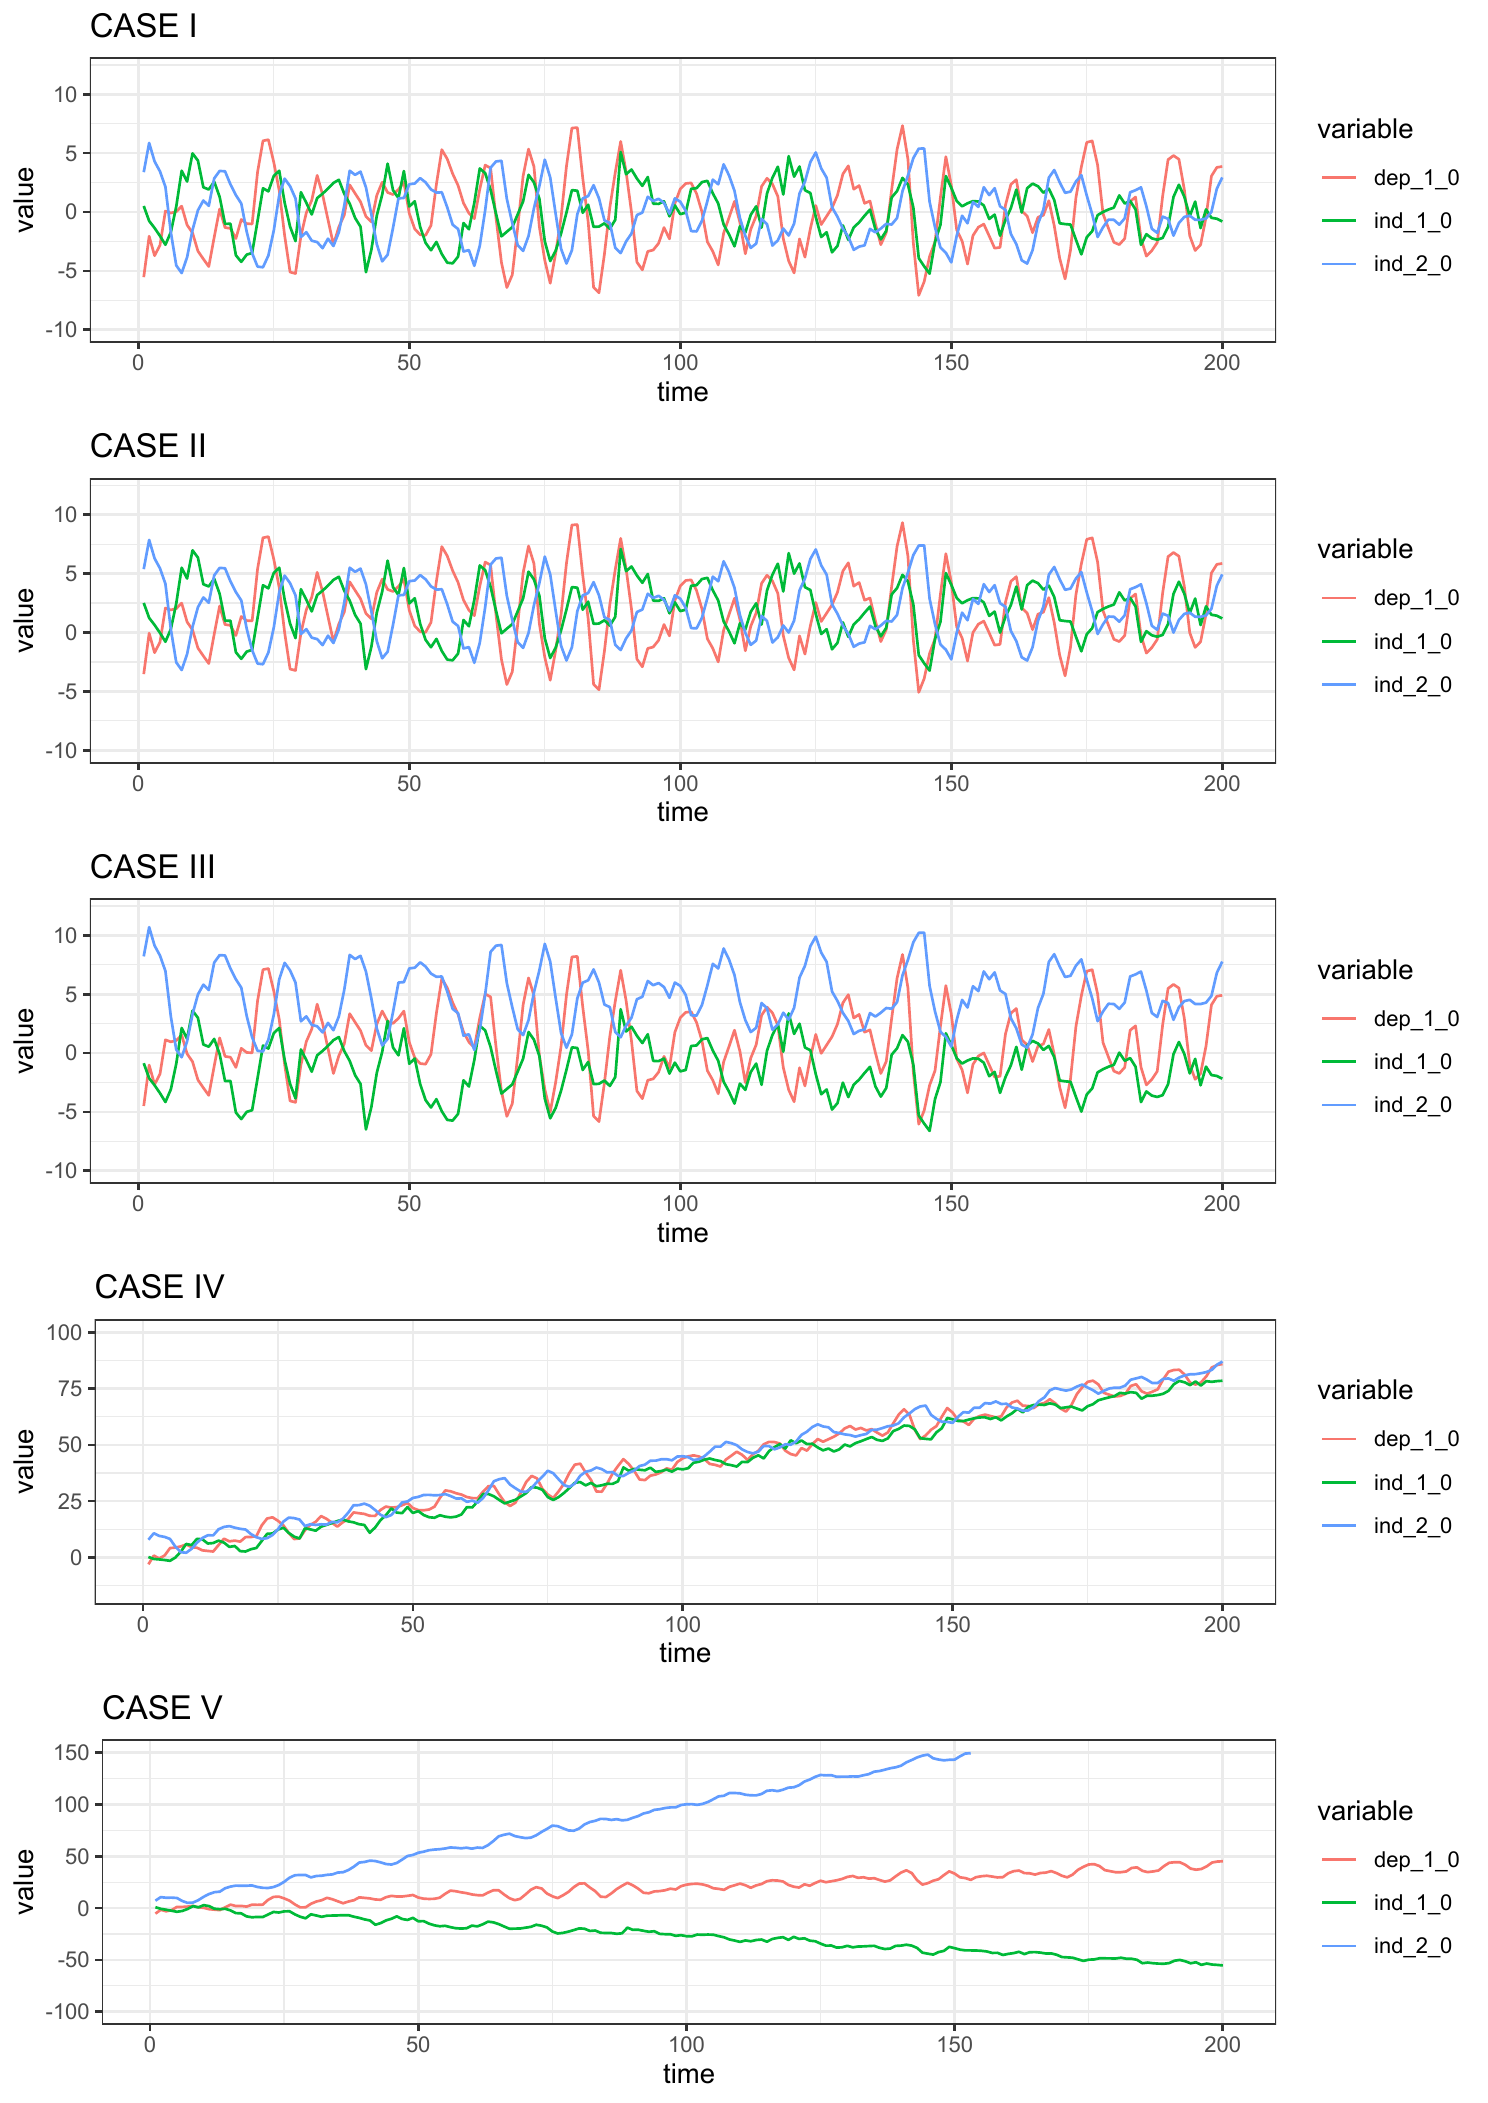
\includegraphics[width=13.5cm]{figures/sim_ts}
\end{center}
\caption{Simulated data from the VECM / conditional ARDL specifications, for every case. Made with \CRANpkg{ggplot} \citep{ggplot}.}
\label{fig:sim}
\end{figure}
\begin{figure}[ht!]
\begin{center}
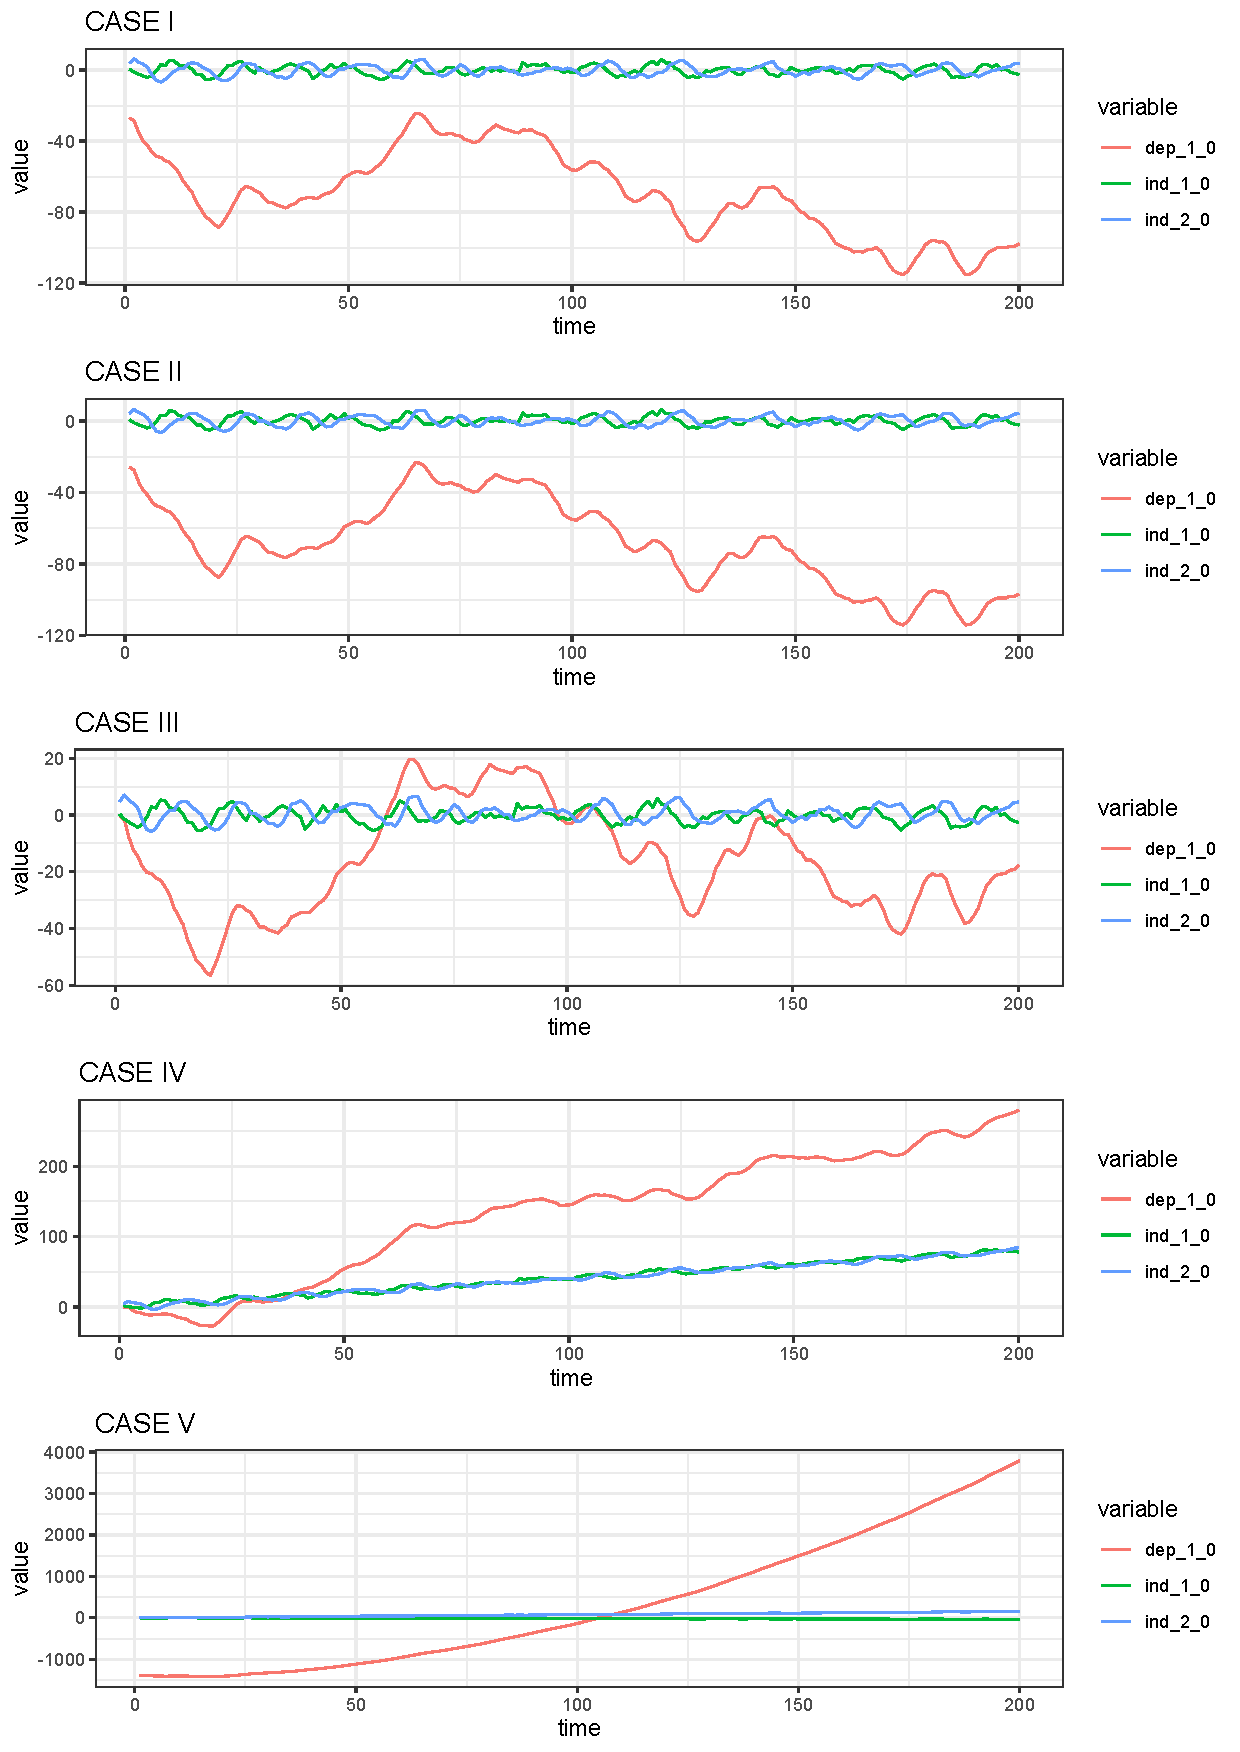
\includegraphics[width=13.5cm]{figures/sim_ts_D2}
\end{center}
\caption{Simulated data from the VECM / conditional ARDL specifications (degenerate case of type 2, $a_{yy}=0$), for every case. Made with \CRANpkg{ggplot}.}
\label{fig:sim2}
\end{figure}
\newpage
\begin{landscape}
\tikzset{
  treenode/.style = {shape=rectangle, rounded corners,
                     draw,align=center,
                     top color=white,
                     text width = 4cm,
                     inner sep=2ex,
                     anchor=center},
  input/.style = {align=center, text width=4.5cm},
  decision/.style = {treenode, diamond, inner sep=3pt},
  action/.style = {treenode, circle, inner sep=1pt,
                     text width = 2.5cm},
  root/.style     = {treenode},
  env/.style      = {treenode},
  ginish/.style   = {root},
  dummy/.style    = {circle,draw},
  ar/.style={->,>=latex}
}
\tikzset{connect/.style={rounded corners=#1,
        to path= ($(\tikztostart)!-#1!(\tikztotarget)!-#1!-90:(\tikztotarget)$) -- ($(\tikztotarget)!-#1!(\tikztostart)!-#1!90:(\tikztostart)$) --
        ($(\tikztotarget)!-#1!(\tikztostart)!#1!90:(\tikztostart)$) -- ($(\tikztostart)!-#1!(\tikztotarget)!-#1!90:(\tikztotarget)$) -- cycle (\tikztotarget)
}}
\tikzset{connect/.default=4mm}
\begin{figure}[ht!]
\centering
\begin{tikzpicture}[-latex][scale=0.3]
  \matrix (chart)
    [
      matrix of nodes,
      column sep      = 2.5em,
      row sep         = 1ex,
      row 2/.style = {nodes={decision}},
      row 5/.style = {nodes={env}}
    ]
    {  %first row
       |[input]| {\small VAR/VECM input\\ $\boldsymbol \mu$, $\boldsymbol \eta$, $\boldsymbol\alpha_0$, $\boldsymbol\alpha_1$, \texttt{case}}
       &
       |[input]| {\small VECM/ARDL input\\ $\mathbf A_{xx},\mathbf a_{yx},a_{yy},\boldsymbol{\Gamma}_j$}&
       \\
       %second row
       |[treenode]|{\scriptsize  VECM
       Intercept and trend\\
       \phantom{x}\\
       CASE I:\\  $\boldsymbol{\mu}=\boldsymbol{\eta}=\mathbf 0\rightarrow
        \boldsymbol\alpha_0 = \boldsymbol\alpha_1 = \mathbf 0$     \\
       \phantom{x}\\
       CASE II:\\ 
       $\boldsymbol{\mu}$ input, $\boldsymbol\eta=\mathbf 0$, $\boldsymbol\alpha_{0} =  \mathbf A(1) \boldsymbol{\mu}$, $\boldsymbol\alpha_1 = \mathbf 0$\\
        \phantom{x}\\
        CASE III:\\
       $\boldsymbol\eta=\mathbf 0 $ \\
       $\boldsymbol{\alpha}_{0}$ input, $\boldsymbol{\alpha}_1 = \mathbf 0$\\ 
       \phantom{x}\\
       CASE IV:\\
       $\boldsymbol{\alpha}_{0}$ input, $\boldsymbol{\eta}$ input, $\boldsymbol{\alpha}_1 =\mathbf A(1)\boldsymbol{\eta}$\\
       \phantom{x}\\
       CASE V:\\
       $\boldsymbol{\alpha}_{0}$ input, $\boldsymbol{\alpha}_1$ input
       \normalsize}&
       |[treenode]| {\small Long-run VECM matrix 
       $\mathbf A = 
       \begin{bmatrix} {a_{yy}} & {\mathbf{a}_{yx}'} \\
       {\mathbf 0} & {\mathbf{A}_{xx}}  
       \end{bmatrix}$.\\
       \phantom{x}\\
       Short-run VECM matrices 
       $\boldsymbol\Gamma_j$ \\
       $\boldsymbol\Gamma(1) = \mathbf{I_K}-\sum_{j=1}^p\boldsymbol\Gamma_j$}&
       |[treenode]|{\scriptsize  ARDL
       Intercept and trend\\
       \phantom{x}\\
       CASE I:\\  $\boldsymbol{\mu}=\boldsymbol{\eta}=\mathbf 0\rightarrow$\\
        $\theta_0=\alpha_{0.y} = \theta_1=\alpha_{1.y} = 0$\\
       \phantom{x}\\
       CASE II:\\
       $\theta_0\neq 0 \enspace \alpha_{0.y} = 0$ (Intercept in $EC$)\\
       $\boldsymbol\eta=\mathbf 0 \rightarrow \theta_1 =\alpha_{1.y}= 0$\\
        \phantom{x}\\
        CASE III:\\
        $\alpha_{0.y}=\alpha_{0y}-\boldsymbol\omega'\boldsymbol\alpha_{0x}$ $(\theta_0 =  0)$\\
       $\boldsymbol\eta=\mathbf 0 \rightarrow \theta_1 =\alpha_{1.y}= 0$\\ 
       \phantom{x}\\
       CASE IV:\\
       $\alpha_{0.y}=\alpha_{0y}-\boldsymbol\omega'\boldsymbol\alpha_{0x}$ $(\theta_0 =  0)$\\
       $\theta_1\neq 0 \enspace \alpha_{1.y} = 0$ (Trend in $EC$)\\
       \phantom{x}\\
       CASE V:\\
       $\alpha_{0.y}=\alpha_{0y}-\boldsymbol\omega'\boldsymbol\alpha_{0x}$ $(\theta_0 =  0)$\\
       $\alpha_{1.y}=\alpha_{1y}-\boldsymbol\omega'\boldsymbol\alpha_{1x}$ $(\theta_1 =  0)$
       \normalsize}
       \\
       %third row
       |[action]| {\small $\boldsymbol{\Sigma}$ input.\\ Error generation\\
       $\mathbf u_t'\sim N_{K+1}(\mathbf 0,\boldsymbol\Sigma)$
       \normalsize}&
       |[action]| {\small Conditioning\\
       $\boldsymbol\omega'=
       \boldsymbol\sigma_{yx}'\boldsymbol\Sigma_{xx}^{-1}$
       \normalsize}&
       |[treenode]|{\small $\mathbf {\tilde{a}}_{y.x}'=\mathbf a_{yx}'-\boldsymbol\omega'\mathbf A_{xx}$\\
       $\widetilde{\mathbf A} =
       \begin{bmatrix}
       {a_{yy}} & \mathbf{\tilde{a}}'_{y.x}\\
       {\mathbf 0} & {\mathbf{A}_{xx}}  
       \end{bmatrix}$\\
       $\boldsymbol\gamma_{y.x,j}=
       \boldsymbol\gamma_{yx}-\boldsymbol\omega'\boldsymbol\Gamma_{(x),j}$\\
       $\widetilde{\boldsymbol\Gamma}_j =
       \begin{bmatrix}
       \boldsymbol{\gamma}_{y.x,j}\\
       \boldsymbol\Gamma_{(x),j}
       \end{bmatrix}$\\
       $\nu_{yt}=\varepsilon_{yt}-\boldsymbol\omega'\boldsymbol\varepsilon_{xt}$
       \normalsize}\\
        |[input]| {\small Other input:\\
        \texttt{nobs}, \texttt{burn.in}}
       &
       |[action]| {\small $\Delta \mathbf x_t$ via \eqref{eq:marg}\\
       $\mathbf x_t = \Delta \mathbf x_t + \mathbf x_{t-1} $\\
       $\Delta y_t$ via \eqref{eq:ardl}\\
       $y_t = \Delta y_t + y_{t-1} $\\
       \normalsize}&\\
       };
       \draw[thick]
		 (chart-1-1) ->  (chart-2-1);
       \draw[thick]
		 (chart-1-2) -> (chart-2-2);
       \draw[thick]
		 (chart-2-2) -> (chart-2-1);
       \draw[thick]
		 (chart-2-1) -> (chart-3-2);
       \draw[thick]
		 (chart-2-2) -> (chart-3-2);
       \draw[thick]
		 (chart-3-1) -> (chart-3-2);
       \draw[thick]
		 (chart-3-2) -> (chart-2-3);
       \draw[thick]
		 (chart-3-2) -> (chart-3-3);
    \begin{scope}[transform canvas={yshift=1.7em}]
       \draw[red,dashed,ultra thick] (chart-2-3) to[connect=29.5mm,rounded corners=2mm] (chart-3-3);
    \end{scope}
    \begin{scope}[transform canvas={yshift=1em}]
       \draw[blue,dashed,ultra thick] (chart-2-1) to[connect=27mm,rounded corners=2mm] (chart-3-1);
    \end{scope}
       \draw[blue,ultra thick,shorten < = 1.85cm] (chart-3-1) edge node[left=0.75cm,pos=0.67]{\small Unconditional parameters for $\Delta\mathbf x_t$\normalsize} (chart-4-2);
       \draw[red,ultra thick,shorten < = 0.75cm] (chart-3-3) edge node[right=1cm,pos=0.5]{\small Conditional parameters for $\Delta y_t$\normalsize} (chart-4-2);
       \draw[thick]
		 (chart-3-2) -> (chart-4-2);
       \draw[thick] (chart-4-2) edge [in=-20, out=20,looseness=3,right=0.2cm] node[right=0.2cm]{\small Until \texttt{nobs+burn.in}. 
       Discard \texttt{burn.in}\normalsize} (chart-4-2);
       \draw[thick]
		 (chart-4-1) -> (chart-4-2);
  \end{tikzpicture}
	\caption{Flowchart of the \texttt{sim\_vecm\_ardl} function inner steps. When applying \eqref{eq:ardl} and \eqref{eq:marg}, $y_{t_j}=0$, $\Delta y_{t_j}=0$, $\mathbf x_{t_j}=\mathbf 0$, $\Delta \mathbf x_{t_j}= \mathbf 0$ for any $t_j < 1$. Boxes denote parameter definitions and transformations. Circles denote crucial actions, Empty nodes denote function inputs.}\label{fig:flowchart}
	\end{figure}
\end{landscape}
\subsection{Bootstrapping the ARDL bound tests: the \code{boot\_ardl} function}
This function develops the bootstrap procedure detailed previously. As an option in the initial estimation phase, it offers the possibility of automatically choosing the best order for the lagged differences of all the variables in the ARDL and VECM models. This is done by using  several criteria. In particular, AIC, BIC, AICc, $R^2$ and $R^2_{adj}$ are used as lag selection criteria for the ARDL model, while the overall minimum between AIC, HQIC, SC and FPE is used for the lag selection for the VECM.\\
In particular, the \code{auto\_ardl} function in the package \CRANpkg{ARDL} \citep{PKGARDL} selects the best ARDL order in terms of the short-run parameter vectors $\boldsymbol\gamma_{y.x,j}$, while the \code{VARselect} function in the package \CRANpkg{vars} \citep{PKGVARS} selects the best VECM order in terms of the short-run parameter matrices $\boldsymbol\Gamma_{(x),j}$. Furthermore, the user can input a significance threshold for the retention of single parameters in the $\boldsymbol\Gamma_j$ and in the $\boldsymbol\gamma_{y.x,j}$ vectors.\\
The function \code{boot\_ardl} takes the following arguments:
\begin{itemize}
\item \code{data}: input dataset. Must contain a dependent variable and a set of independent variables;
\item \code{yvar}: name of the dependent variable enclosed in quotation marks. If unspecified, the first variable in the dataset is used;
\item \code{xvar}: vector of names of the independent variables, each enclosed in quotation marks. If unspecified, all variables in the dataset except the first are used;
\item \code{fix.ardl}: vector $(j_1,\dots,j_K)$, containing the maximum orders of the lagged differences (i.e., $\Delta y_{t-j_1}, \Delta x_{1,t-j_2},\dots,$ $\Delta x_{1,t-j_K}$) for the short term part of the ARDL equation, chosen in advance; 
\item \code{info.ardl}: (alternatively to \code{fix.ardl}) the information criterion used to choose the best lag order for the short term part of the ARDL equation. It must be one between \code{AIC} (default), \code{AICc}, \code{BIC}, \code{R2}, , \code{adjR2}; 
\item \code{fix.vecm}: scalar $m$ containing the maximum order of the lagged differences (i.e., $\Delta\mathbf z_{t-m}$) for the short term part of the VECM equation, chosen in advance; 
\item \code{info.vecm}: (alternatively to \code{fix.vecm}) the information criterion used to choose the best lag order for the short term part of the VECM equation. Must be one among \code{AIC} (default), \code{HQIC}, \code{SC}, \code{FPE}; 
\item \code{maxlag}: (in conjunction with \code{info.ardl} / \code{info.vecm}) maximum number of lags for the \code{auto\_ardl} function in the package \CRANpkg{ARDL}, and for the \code{VARselect} function in the package \CRANpkg{vars};
\item \code{a.ardl}: significance threshold for the short-term ARDL coefficients ($\boldsymbol\gamma_{y.x,j}$) in the ARDL model estimation; 
\item \code{a.vecm}: significance threshold for the short-term VECM coefficients (in $\boldsymbol\Gamma_j$) in the VECM model estimation;
\item \code{nboot}: number of bootstrap replications;
\item \code{case}: type of the specification for the conditional ARDL in terms of deterministic components (intercept and trend) among the five proposed by \cite{pesaran2001}, given in \eqref{eq:case1}-\eqref{eq:case5};
\item \code{a.boot.H0}: probability/ies $\alpha$ by which the critical quantiles of the bootstrap distribution(s) $c^{*}_{\alpha,F_{ov}}$, $c^{*}_{\alpha,t}$ and $c^{*}_{\alpha,F_{ind}}$ must be calculated;
\item \code{print}: if set to \code{TRUE}, shows the progress bar.
\end{itemize}
\code{boot\_ardl} makes use of the \code{lag\_mts} function which produces lagged versions of a given matrix of time series, each column with a separate order. \code{lag\_mts}  takes as parameters the data included in a matrix \code{X} and the lag orders in a vector \code{k}, with the addition of a boolean parameter \code{last.only}, which allows to specify whether only the $k$-th order lags have to be retained, or all the lag orders from the first to the $k$-th.\\
\code{boot\_ardl} also acts as a wrapper for the most common methodologies detecting cointegration, offering a comprehensive view on the testing procedures involved in the analysis.
The resulting object, of class \code{bootCT}, contains all the information about
\begin{itemize}
\item The conditional ARDL model estimates, and the unconditional VECM model estimates;
    \item the bootstrap tests performed in the conditional ARDL model;
     \item the Pesaran, Shin and Smith bound testing procedure ($F_{ov}$ and $t$-test, when applicable);
    \item the Sam, McNown and Goh bound testing procedure for $F_{ind}$, when applicable;
    \item the Johansen rank and trace cointegration tests on the independent variables.
    \end{itemize}
    Internally, the bootstrap data generation under the null is executed via a \code{Rcpp} function, employing the \CRANpkg{Rcpp} and \CRANpkg{RcppArmadillo} packages \citep{RCPP}, so as to greatly speed up computational times.
    As explained in the previous section, cointegration tests in the unconditional ARDL model are performed in order to uncover the presence of spurious cointegrating relationships.\\   
To this end, the function provides
    \begin{itemize}
    \item the bootstrap critical values of the $F_{ov}$, $t$ and $F_{ind}$ tests in the conditional model, at level \code{a.boot.H0}, along with the same statistics computed in the conditional model.
    \item a flag, called \code{fakecoint}, that indicates divergence between the outcomes of the $F_{ind}$ test performed in both the conditional and unconditional model. In this circumstance, as explained before, there is no cointegration \citep[see][]{bertelli2022bootstrap}.
\end{itemize}
A \code{summary} method has been implemented to present the results in a visually clear manner. It accepts the additional argument "\code{out}" that lets the user choose which output(s) to visualize: \code{ARDL} prints the conditional ARDL model summary, \code{VECM} prints the VECM model summary, \code{cointARDL} prints the summary of the bound tests and the bootstrap tests, \code{cointVECM} prints the summary of the Johansen test on the independent variables.\\
A detailed flowchart showing the function's workflow is displayed in Figure \ref{fig:flowchart_ardl}. There, the expressions "C ARDL" and "UC ARDL" stand for conditional and unconditional ARDL model, respectively.\\
\newpage
\begin{landscape}
\tikzset{
  treenode/.style = {shape=rectangle, rounded corners,
                     draw,align=center,
                     top color=white,
                     text width = 4.1cm,
                     inner sep=2ex,
                     anchor=center},
  treenodel/.style = {shape=rectangle, rounded corners,
                     draw,align=center,
                     top color=white,
                     text width = 2.2cm,
                     inner sep=2ex,
                     anchor=center},
  input/.style = {align=center, text width=4.5cm},
  decision/.style = {treenode, diamond, inner sep=2pt,
                    text width=2cm},
   decisionx/.style = {treenode, diamond, inner sep=2pt,
                    text width=1.5cm},
  decisiond/.style = {treenode, diamond, dashed, inner sep=3pt,
                    text width=2cm},
  treeuc/.style = {treenode,draw=blue,thick},
  treec/.style = {treenode,draw=red,thick},
  treeg/.style = {treenode,draw=green!60,thick,fill=green!5},
  action/.style = {treenode, circle, inner sep=1pt,
                     text width = 3cm},
  root/.style     = {treenode},
  env/.style      = {treenode},
  ginish/.style   = {root},
  dummy/.style    = {circle,draw},
  ar/.style={->,>=latex}
}
\tikzset{connect/.style={rounded corners=#1,
        to path= ($(\tikztostart)!-#1!(\tikztotarget)!-#1!-90:(\tikztotarget)$) -- ($(\tikztotarget)!-#1!(\tikztostart)!-#1!90:(\tikztostart)$) --
        ($(\tikztotarget)!-#1!(\tikztostart)!#1!90:(\tikztostart)$) -- ($(\tikztostart)!-#1!(\tikztotarget)!-#1!90:(\tikztotarget)$) -- cycle (\tikztotarget)
}}
\tikzset{connect/.default=4mm}

\begin{figure}[ht!]
\centering
\hspace*{-2cm}
\begin{tikzpicture}[-latex][scale=0.3]
  \matrix (chart)[ampersand replacement=\#]
    [
      matrix of nodes,
      column sep      = 1.7em,
      row sep         = 1.5ex,
      row 2/.style = {nodes={decision}},
      row 5/.style = {nodes={env}}
    ]
    {  %first row
       \#
       |[input]| {\small \texttt{case}, \texttt{fix.vecm},\\
       \texttt{info.vecm}, \texttt{maxlag}}\#
       |[input]| {\small \texttt{data},\\
       \texttt{xvar}, \texttt{yvar}}\#
       |[input]|{\small{\texttt{case}, \texttt{fix.ardl},\\
       \texttt{info.ardl}, \texttt{maxlag}}}
       \#
       \\
       %second row
       |[decision]|{\small
       VECM\\Estimate}
       \normalsize\#
       |[treenode]| {\small
       \centering
       \begin{tabular}{c|c}
       \multicolumn{2}{c}{VECM estimation (either)}\\
        Fixed order & \texttt{VARselect()}\\\hline
        \texttt{fix.vecm} & \texttt{info.vecm}    \\
        &\texttt{maxlag}\\
       \end{tabular}}
       \normalsize\#
       |[decisiond]|{\small
       Compute $F_{ind}$ of \\UC ARDL
       \normalsize}
       \#
       |[treenode]| {\small
       \begin{tabular}{c|c}
       \multicolumn{2}{c}{ARDL estimation (either)}\\
        Fixed order & \texttt{auto\_ardl()}\\\hline
        \texttt{fix.ardl} & \texttt{info.ardl}\\
        &\texttt{maxlag}\\
       \end{tabular}}
       \#
       |[decision]|{\small
       C ARDL\\Estimate}
       \normalsize
       \\
       %third row
       |[decision]|{\small
       Johansen test\\
       results on $\mathbf x_t$}
       \normalsize\#
       |[treeuc]| {\scriptsize
       Estimation of the parameters:\\
       $\mathbf A$, $\boldsymbol\Gamma_j$ $(j=1,\dots,p)$\\
       $\boldsymbol\alpha_0$, $\boldsymbol\alpha_1$  based on \texttt{case}. \\       $\widehat{\boldsymbol\varepsilon}_{xt}$ obtained via \eqref{eq:resvecm}.\\
       Significant estimates of $\boldsymbol\Gamma_j$ filtered via \texttt{a.vecm}}
       \normalsize\#
       |[treenode]|{\scriptsize
        Combine to get \\
        $\widetilde{\mathbf A} =
       \begin{bmatrix}
       \color{red}{a_{yy}} & \color{red} \widetilde{\mathbf{a}}'_{y.x}\\
       {\mathbf 0} & \color{blue}{\mathbf{A}}_{xx}  
       \end{bmatrix}$\\
       $\widetilde{\boldsymbol\Gamma}_j =\begin{bmatrix}\color{red}\boldsymbol{\gamma}_{y.x,j}\\
       \color{blue}\boldsymbol\Gamma_{(x),j}
       \end{bmatrix}$\\
       \phantom{\tiny x}\\
       $\boldsymbol{\omega}$ (only in the C ARDL)\\
       $(\boldsymbol\alpha_{0}^{c})' = [\color{red}{\alpha_{0.y}}\;\color{blue}{\boldsymbol\alpha_{0x}'}]$, $(\boldsymbol\alpha_{1}^{c})' = [\color{red}{\alpha_{1.y}}\;\color{blue}{\boldsymbol\alpha_{1x}'}]$
       \normalsize}
       \#
       |[treec]| {\scriptsize
       Estimation of:\\
       $ a_{yy}, \mathbf{a}_{y.x}$, $\boldsymbol\gamma_{y.x,j}$ $(j=1,\dots,p)$\\
       $\boldsymbol\omega$ (only in the C ARDL )\\
              $\alpha_{0.y}$,$\alpha_{1.y}$ based on \texttt{case}.\\
       Significant estimates of $\boldsymbol\gamma_{y.x,j}$ filtered via \texttt{a.ardl}}
       \normalsize
       \#
       |[decisionx]|{\scriptsize
        PSS/SMG results
        in the C ARDL.
       Compute\\ $F_{ov}$, $t$, $F_{ind}$}
       \normalsize
       \\
       \#
       |[treenode]|{\scriptsize
       Null elements of $\widetilde{\mathbf A}$ based on $H_0$.\\
       Nullity of $\boldsymbol\alpha_0^c$ and $\boldsymbol\alpha_1^c$ based on \texttt{case}.\\
       Combine the residuals \\
       $\widehat{\mathbf u}_t = [\color{red}\widehat{\nu}_{yt}^{*}\,\color{blue}\widehat{\boldsymbol\varepsilon}_{xt}]$}
       \#
       |[treec]|
       { $F_{ov}$ test \\
       \small$H_0: a_{yy}=0,\; \widetilde{\mathbf{a}}_{y.x}=\mathbf 0$:\\
       Re-estimate ARDL, obtain\\
       $\widehat{\nu}_{yt}^{F_{ov}}$ via \eqref{eq:resfov}
       \normalsize}
       \#
       |[treec]|{\small $t$-test \\$H_0: a_{yy}=0$:\\
       Re-estimate ARDL, obtain\\
       $\widehat{\nu}_{yt}^{t}$ via \eqref{eq:rest}
       \normalsize}
       \#
       |[treec]|{\small $F_{ind}$ test \\$H_0: \widetilde{\mathbf{a}}_{y.x}=\mathbf 0$:\\
       Re-estimate ARDL, obtain\\
       $\widehat{\nu}_{yt}^{F_{ind}}$ via \eqref{eq:resfind}
       \normalsize}
       \\
       |[treenodel]| {\small Sample and \\center
       from $\widehat{\mathbf U}$.\\
       Get ${\mathbf U^{(b)}}$.
       \normalsize}
       \#
       |[treenode]|{\small $\Delta y_t^{(b)}$, $\Delta\boldsymbol x_t^{(b)}$  via (\ref{eq:resfov}-\ref{eq:rest}-\ref{eq:resfind}-\ref{eq:resvecm})\\
       $\mathbf{x}_t^{(b)}=\Delta\boldsymbol x_t^{(b)} + \mathbf{x}_{t-1}^{(b)}$.
       \\
       ${y}_t^{(b)}=\Delta y_t^{(b)} +y_{t-1}^{(b)}$}
       \#
       |[treenode]|{\small ARDL estimation under $H_0$.\\
       Get $F_{ov}^{(b),H_0}$, $t^{(b),H_0}$,\\ $F_{ind}^{(b),H_0}$ (C) and $F_{ind}^{(b),H_0}$ (UC)}
       \#
       |[decisionx]|{\small $c_{\alpha,T}^*$ at level \texttt{a.boot.H0}.}
       \#
       |[treeg]|{\small Decide comparing \\ $F_{ov}$, $t$, $F_{ind}$ each to its $c_{\alpha,T}^{*}$.\\
       \textbf{IF} $F_{ind}>c_{\alpha,F_{ind}}^{*}$ (C)\\
       \textbf{AND} $F_{ind}<c_{\alpha,F_{ind}}^{*}$ (UC)\\
       $\rightarrow$\textbf{No real cointegration}}
       \\
       };
       \draw[thick]
		 (chart-1-3) ->  (chart-2-2);
       \draw[thick]
		 (chart-1-3) -> (chart-2-4);
       \draw[thick]
		 (chart-1-2) -> (chart-2-2);
       \draw[thick]
		 (chart-1-4) -> (chart-2-4);
       \draw[thick]
		 (chart-2-2) -> (chart-2-1);
       \draw[thick]
		 (chart-2-4) -> (chart-2-5);
       \draw[thick]
		 (chart-2-2.south west) -> (chart-3-1);
       \draw[thick]
		 (chart-2-2) -> (chart-3-2);
       \draw[thick]
		 (chart-2-4.south east) to node[right=0.4cm,pos=-0.1,rotate=-39]{\small Based on \texttt{case}} (chart-3-5);
       \draw[ar,thick]
		 ([xshift=-1 cm]chart-2-4.south) to node[left=0.1cm] {\small UC} ([xshift=-1 cm] chart-3-4.north);
       \draw[ar,thick]   ([xshift=1 cm]chart-2-4.south) to node[right=0.1cm] {\small C} ([xshift=1cm] chart-3-4.north);
   \draw[thick] (chart-2-4) edge [in=70, out=40,looseness=2,left=2cm] node[pos=0.3,right=0.1cm]{\small UC and C model\normalsize} (chart-2-4);
   \draw[thick]
		 (chart-2-4) -> (chart-2-3);
   \draw[blue,ultra thick] (chart-3-2) -> (chart-3-3);
   \draw[red,ultra thick]  (chart-3-4) -> (chart-3-3);
   \draw[red,ultra thick]  (chart-3-4) -> (chart-4-3.north east);
   \draw[red,ultra thick]  (chart-3-4) -> (chart-4-4);
   \draw[red,ultra thick]  (chart-3-4) -> (chart-4-5.north west);
   \draw[blue,ultra thick]  (chart-3-2) -> (chart-4-2);
   \draw[thick] (chart-3-3) -> (chart-4-2);
   \draw[red,ultra thick, shorten < = 0.15cm]  (chart-4-3) -> (chart-4-2);
   
       \begin{scope}[transform canvas={yshift=0em,xshift=3.4em}]
       \draw[red,dashed,ultra thick] (chart-4-3.west) to[connect=13mm,rounded corners=1mm] (chart-4-5);
    \end{scope}
\draw[thick] (chart-4-2.west) -> (chart-5-1.north);
\draw[thick] (chart-5-1) -> (chart-5-2);
\draw[thick] (chart-5-2) -> (chart-5-3);
\draw[thick] (chart-5-3) -> (chart-5-4);
\draw[ar,thick] (chart-5-3.south west) to [bend left=30] node[right=0.4cm,pos=0.2]{\small $b=1,\dots,B$}(chart-5-1.south east);
  \end{tikzpicture}
	\caption{Flowchart of the \texttt{boot\_ardl} function inner steps. Boxes denote parameter definitions and transformations. Diamonds denote function outputs. Dashed diamonds denote intermediate output (not shown after function call). Empty nodes denote function inputs. The first $p+1$ rows of $\mathbf z_t^{(b)}$ are set equal to the first $p+1$ rows of the original data. The best lag order for each difference variable in the ARDL model is determined via \texttt{auto\_ardl()}. It is reported as a unique value $p$ in $\boldsymbol{\gamma}_{y.x,j}$ for brevity in the flowchart.}\label{fig:flowchart_ardl}
	\end{figure}
\end{landscape}
\subsection{Execution time and technical remarks}
In order to investigate the sensitivity of the procedure to different sample sizes and number of bootstrap replicates, an experiment has been run using a three-dimensional time series of length $T=\{50,80,100,200,500\}$, generating 100 datasets for each sample size with the \code{sim\_vecm\_ardl} function (Case II, with cointegrated variables, and 2 lags in the short-run section of the model).\\ Then, the \code{boot\_ardl} function has been called

\begin{example}
boot_ardl(data = df_sim,
          nboot = bootr,
          case = 2,
          fix.ardl = rep(2, 3),
          fix.vecm = 2)
\end{example}

\noindent In the code above, \code{bootr} has been set equal to $B=\{200,500,1000,2000\}$, the number of lags has been assumed known (\code{fix.ardl} and \code{fix.vecm}), while default values have been used for every other argument (such as \code{a.ardl}, \code{a.vecm} and \code{a.boot.H0}).\\
Table \ref{tab:exec} shows the average running time per replication together with  the coefficient of variation (\%) of the bootstrap critical values of the $F_{ov}$ test, for each value of $T$ and $B$, across 100 replications for each scenario.\\
Naturally, the running time increases as both sample size and bootstrap replicates increase. However, it can be noticed how the coefficients of variation tend to stabilize for $B \geq 1000$, especially for $T>80$, at the 5\% significance level. Therefore, it is recommended a number of bootstrap replicates of at least $B=1000$ for higher sample size, or at least $B=2000$ for smaller samples. The analysis has been carried out using an Intel(R) Core(TM) i7-1165G7 CPU @ 2.80GHz processor, 16GB of RAM.

\begin{table}[htbp]
  \centering
    \begin{tabular}{cccccc}
    \multicolumn{1}{c}{$T$} & \multicolumn{1}{l}{$B$} & \multicolumn{1}{c}{Exec. Time (sec)} & \multicolumn{1}{c}{$cv^{(F_{ov})}(5\%)$} & \multicolumn{1}{c}{$cv^{(F_{ov})}(2.5\%)$} & \multicolumn{1}{c}{$cv^{(F_{ov})}(1\%)$} \\
    \midrule
    50    & 200   & 23.38 & 8.648 & 10.925 & 13.392 \\
    50    & 500   & 48.37 & 6.312 & 6.952 & 8.640 \\
    50    & 1000  & 96.65 & 4.806 & 5.613 & 6.288 \\
    50    & 2000  & 231.15 & 4.255 & 4.226 & 4.946 \\
    \midrule
    80    & 200   & 23.46 & 7.251 & 8.936 & 11.263 \\
    80    & 500   & 50.19 & 4.998 & 6.220 & 7.946 \\
    80    & 1000  & 143.00 & 3.882 & 4.453 & 5.305 \\
    80    & 2000  & 255.64 & 2.912 & 3.623 & 4.518 \\
    \midrule
    100   & 200   & 37.89 & 7.707 & 8.583 & 10.955 \\
    100   & 500   & 52.86 & 4.691 & 5.304 & 7.557 \\
    100   & 1000  & 184.51 & 3.512 & 4.567 & 5.695 \\
    100   & 2000  & 212.65 & 3.519 & 3.674 & 4.185 \\
    \midrule
    200   & 200   & 35.46 & 6.644 & 7.173 & 10.365 \\
    200   & 500   & 76.78 & 4.734 & 5.355 & 6.225 \\
    200   & 1000  & 148.25 & 3.124 & 4.177 & 5.034 \\
    200   & 2000  & 484.51 & 2.811 & 3.361 & 3.907 \\
    \midrule
    500   & 200   & 54.47 & 6.641 & 8.694 & 10.414 \\
    500   & 500   & 133.17 & 5.137 & 5.816 & 6.408 \\
    500   & 1000  & 271.87 & 3.905 & 4.585 & 5.283 \\
    500   & 2000  & 561.71 & 3.221 & 3.490 & 4.145 \\
    \bottomrule
    \end{tabular}%
     \caption{Average execution times (in seconds) of the \code{boot\_ardl} function, for different combinations of sample size $T$ and bootstrap replicates $B$. Coefficients of variation ($cv$) reported for the $F_{ov}$ bootstrap critical values at level 5\%, 2.5\% and 1\%.}
  \label{tab:exec}%
\end{table}%

\section{Empirical applications}\label{sec:app}
This section provides two illustrative application which highlight the performance of the bootstrap ARDL tests.
\subsection{An application to the German macroeconomic dataset}
In the first example, the occurrence of a long-run relationship between consumption [C], income [INC], and investment [INV] of Germany has been investigated via a set of ARDL models, where each variable takes in turn the role of dependent one, while the remaining are employed as independent.
   The models have been estimated by employing the dataset of \citet{lutkepohl2005} which includes quarterly data of the series over the years 1960 to 1982.
    The data have been employed in logarithmic form. Figure \ref{fig:plotemp} displays these series over the sample period.\\
    Before applying the bootstrap procedure, the order of integration of each series has been analyzed. Table \ref{tab:adf} shows the results of ADF test performed  on  both the series and their first-differences ($k=3$ maximum lags). The results confirm the applicability of the ARDL framework as no series is integrated of order higher than one.\\
    The following ARDL equations have been estimated:
\begin{enumerate}[I]
    \item First ARDL equation (C | INC, INV):
    \begin{align}
    \Delta \log \text{C}_{t}&=\alpha_{0.y} -
    a_{yy} \log \text{C}_{t-1} - {a}_{y.x_1}\log \text{INC}_{t-1} - {a}_{y.x_2}\log \text{INV}_{t-1} +\\\nonumber
    &\sum_{j=1}^{p-1}\gamma_{y.j} \Delta\log \text{C}_{t-j} +
    \sum_{j=1}^{s-1}\gamma_{x_1.j} \Delta\log \text{INC}_{t-j} +
    \sum_{j=1}^{r-1}\gamma_{x_2.j} \Delta\log \text{INV}_{t-j} +\\\nonumber
    &\omega_1 \Delta\log \text{INC}_{t}+
    \omega_2 \Delta\log \text{INV}_{t}+\nu_{t}. 
    \end{align}

    \item Second ARDL equation (INC | C, INV):
    \begin{align}
    \Delta \log \text{INC}_{t}&=\alpha_{0.y} -
    a_{yy} \log \text{INC}_{t-1} - {a}_{y.x_1}\log \text{C}_{t-1} - {a}_{y.x_2}\log \text{INV}_{t-1} +\\\nonumber
    &\sum_{j=1}^{p-1}\gamma_{y.j} \Delta\log \text{INC}_{t-j} +
    \sum_{j=1}^{s-1}\gamma_{x_1.j} \Delta\log \text{C}_{t-j} +
    \sum_{j=1}^{r-1}\gamma_{x_2.j} \Delta\log \text{INV}_{t-j} +\\\nonumber
    &\omega_1 \Delta\log \text{C}_{t}+
    \omega_2 \Delta\log \text{INV}_{t}+\nu_{t}. 
    \end{align}

    \item Third ARDL equation (INV | C, INC):
    \begin{align}
    \Delta \log \text{INV}_{t}&=\alpha_{0.y} -
    a_{yy} \log \text{INV}_{t-1} - {a}_{y.x_1}\log \text{C}_{t-1} - {a}_{y.x_2}\log \text{INC}_{t-1} +\\\nonumber
    &\sum_{j=1}^{p-1}\gamma_{y.j} \Delta\log \text{INV}_{t-j} +
    \sum_{j=1}^{s-1}\gamma_{x_1.j} \Delta\log \text{C}_{t-j} +
    \sum_{j=1}^{r-1}\gamma_{x_2.j} \Delta\log \text{INC}_{t-j} +\\\nonumber
    &\omega_1 \Delta\log \text{C}_{t}+
    \omega_2 \Delta\log \text{INC}_{t}+\nu_{t}. 
    \end{align}

\end{enumerate}

\noindent Table \ref{tab:est} shows the estimation results for each  ARDL and VECM model. It is worth noting that the instantaneous difference of the independent variables are highly significant in each conditional ARDL model.
Thus, neglecting these variables in the ARDL equation, as happens in the unconditional version of the model, may potentially lead to biased estimates and incorrect inference.
For the sake of completeness, also the results of the marginal VECM estimation are reported for each model.\\
The code to prepare the data, available in the package as the \code{ger\_macro} dataset, is:
\begin{example}
    data("ger_macro")
    LNDATA = apply(ger_macro[,-1], 2, log)
    col_ln = paste0("LN", colnames(ger_macro)[-1])
    LNDATA = as.data.frame(LNDATA)
    colnames(LNDATA) = col_ln
\end{example}

\noindent Then, the \code{boot\_ardl} function is called, to perform the bootstrap tests. In the code chunk below, Model I is considered.

\begin{example}
    set.seed(999)
    BCT_res_CONS = boot_ardl(data = LNDATA,
                         yvar = "LNCONS",
                         xvar = c("LNINCOME", "LNINVEST"),
                         maxlag = 5,
                         a.ardl = 0.1,
                         a.vecm = 0.1,
                         nboot = 2000,
                         case = 3,
                         a.boot.H0 = c(0.05),
                         print = T)
\end{example}
to which follows the call to the \code{summary} function
\begin{example}
    summary(BCT_res_CONS, out = "ARDL")
    summary(BCT_res_CONS, out = "VECM")
    summary(BCT_res_CONS, out = "cointVECM")
    summary(BCT_res_CONS, out = "cointARDL")
\end{example}
The first summary line displays the output in the ARDL column of Table \ref{tab:est} and the second column of Table \ref{tab:cointbig}, Model I. The second line corresponds to the VECM columns of Table \ref{tab:est}, Model I - only for the independent variables. The information on the rank of the $\mathbf A_{xx}$ in Table \ref{tab:est} is inferred from the third line. Finally, the fourth summary line corresponds to the test results in Table \ref{tab:cointbig}, Model I.
A textual indication of the presence of spurious cointegration is displayed at the bottom of the \code{"cointARDL"} summary, if detected.\\
In this example, the bootstrap and bound testing procedures are in agreement only for model I, indicating the existence of a cointegrating relationship. Additionally, no spurious cointegration is detected for this model. As for models II and III, the null hypothesis is not rejected by the bootstrap tests, while the PSS and SMG bound tests fail to give a conclusive answer in the $F_{ind}$ test.\\
The running time of the entire analysis is of roughly 11 minutes, using an Intel(R) Core(TM) i7-1165G7 CPU @ 2.80GHz processor, 16GB of RAM.

\begin{center}
\begin{table}[htbp]
\centering
  \resizebox{0.65\textwidth}{!}{
    \begin{tabular}{crrrrr}
          &       & \multicolumn{2}{c}{level variable} & \multicolumn{2}{c}{first difference} \\
\cmidrule{3-6}    Series & \multicolumn{1}{c}{lag} & \multicolumn{1}{c}{ADF} & \multicolumn{1}{c}{p.value} & \multicolumn{1}{c}{ADF} & \multicolumn{1}{c}{p-value} \\
    \midrule
    \multirow{4}{*}{$\log\text{C}_t$} 
          & 0     & -1.690 & 0.450 & -9.750 & $< 0.01$ \\
          & 1     & -1.860 & 0.385 & -5.190 & $< 0.01$ \\
          & 2     & -1.420 & 0.549 & -3.130 & 0.030 \\
          & 3     & -1.010 & 0.691 & -2.720 & 0.080 \\
    \midrule
    \multirow{4}{*}{$\log\text{INC}_t$} 
          & 0     & -2.290 & 0.217 & -11.140 & $<0.01$ \\
          & 1     & -1.960 & 0.345 & -7.510 & $< 0.01$ \\
          & 2     & -1.490 & 0.524 & -5.120 & $< 0.01$ \\
          & 3     & -1.310 & 0.587 & -3.290 & 0.020 \\
    \midrule
    \multirow{4}{*}{$\log\text{INV}_t$} 
          & 0     & -1.200 & 0.625 & -8.390 & $< 0.01$ \\
          & 1     & -1.370 & 0.565 & -5.570 & $< 0.01$ \\
          & 2     & -1.360 & 0.570 & -3.300 & 0.020 \\
          & 3     & -1.220 & 0.619 & -3.100 & 0.032 \\
    \bottomrule
    \end{tabular}
  }
    \caption{ADF preliminary test (null hypothesis: random walk with drift).}
  \label{tab:adf}
\end{table}%
\end{center}
\begin{center}
\begin{figure}[htbp!]
        \centering
        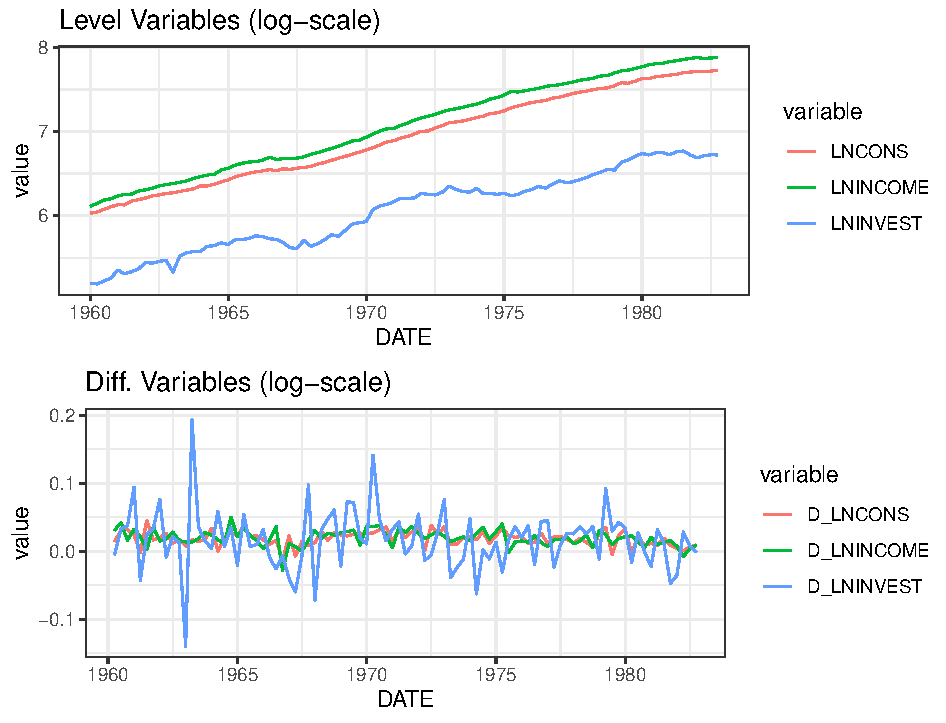
\includegraphics[scale=0.8]{figures/tsgraph.pdf}
        \caption{log-consumption/investment/income graphs (level variables and first differences). Made with \CRANpkg{ggplot}.}
        \label{fig:plotemp}

\end{figure}
\end{center}

\begin{landscape}
\begin{table}[ht!]
\resizebox{1.6\textwidth}{!}{
\begin{tabular}{c lll lll lll}

&
\multicolumn{3}{c}{Model I}&
\multicolumn{3}{c}{Model II}&
\multicolumn{3}{c}{Model III}\\

\cmidrule{2-10}
& \multicolumn{1}{c}{ARDL} & \multicolumn{2}{c}{VECM}
& \multicolumn{1}{c}{ARDL} & \multicolumn{2}{c}{VECM}
& \multicolumn{1}{c}{ARDL} & \multicolumn{2}{c}{VECM}\\

& \multicolumn{1}{c}{$\Delta\log\text{C}_t$} & \multicolumn{1}{c}{$\Delta\log\text{INV}_t$} & \multicolumn{1}{c}{$\Delta\log\text{INC}_t$}
& \multicolumn{1}{c}{$\Delta\log\text{INC}_t$} & \multicolumn{1}{c}{$\Delta\log\text{C}_t$} & \multicolumn{1}{c}{$\Delta\log\text{INV}_t$}
& \multicolumn{1}{c}{$\Delta\log\text{INV}_t$}  & \multicolumn{1}{c}{$\Delta\log\text{C}_t$} & \multicolumn{1}{c}{$\Delta\log\text{INC}_t$}\\

    \midrule
    
    $\log\text{C}_{t-1}$ &
    \makecell{-0.307 ***\\ (0.055)} & & &
    \makecell{0.168 *\\ (0.081)} & \makecell{-0.0011\\ (0.0126)}& \makecell{0.1286*\\ (0.0540)}&  
    \makecell{0.611 . \\ (0.339)}&
    \makecell{-0.2727***\\ (0.0704)} & \makecell{-0.0508\\ (0.0796)} \\
    
    $\log\text{INC}_{t-1}$ &
    \makecell{0.297 ***\\ (0.055)} & \makecell{0.124 *\\ (0.054)} & \makecell{-0.017\\ (0.014)} &
    \makecell{-0.183*\\ (0.079)} &  & &
    \makecell{-0.491\\ (0.340)}  &
    \makecell{ 0.2619***\\ (0.0681)}&\makecell{ 0.0464\\ (0.0772)}\\
    
    $\log\text{INV}_{t-1}$ &
    \makecell{-0.001\\ (0.011)}  & \makecell{-0.152 *\\ (0.063)} & \makecell{0.016\\ (0.017)} &
    \makecell{0.0209\\ (0.0135)} & \makecell{-0.00107\\ (0.0142)} & \makecell{-0.1531*\\ (0.0607)}   &
    \makecell{-0.1212*\\ (0.060)}  & & \\
    
    \midrule
    
    $\Delta\log\text{C}_{t-1}$ &
    \makecell{-0.248 **\\ (0.079)}  & \makecell{0.899 *\\ (0.442)} & \makecell{0.211 .\\ (0.113)}&
    \makecell{0.375***\\ (0.1086)} &  &\makecell{0.9288*\\ (0.442)} &
    \makecell{1.113 *\\ (0.441)}&
    &  \makecell{0.2072 . \\ (0.1142)}\\
    
    $\Delta\log\text{C}_{t-2}$
    & & \makecell{0.744 \\ (0.431)} & & & & \makecell{0.8049 . \\ (0.4345)}& & & \\
    
    $\Delta\log\text{INC}_{t-1}$ &
    & & & \makecell{-0.1404\\ (0.1095)} &  & &
    & & \\
    
    $\Delta\log\text{INC}_{t-2}$ &
    & & 
    & &\makecell{0.2675**\\ (0.0958)} &
    & &\makecell{0.1522.\\ (0.0912)} & \\
    
    $\Delta\log\text{INV}_{t-1}$ &
    & \makecell{-0.18\\ (0.111)} & \makecell{0.035\\ (0.029)} &
    & & \makecell{-0.189 . \\ (0.1097)} &
    \makecell{-0.175\\ (0.1075)} &
    &  \makecell{0.0479 . \\ (0.0282)} \\
    
    $\Delta\log\text{INV}_{t-2}$ &
     & &
    \makecell{0.049 .\\ (0.027) }& & \makecell{0.0591*\\ (0.0245) }&
    & &\makecell{0.0578*\\ (0.0223) } & \makecell{0.0562*\\ (0.0266)} \\
    
    \midrule
    
    $\Delta\log\text{C}_t$ &
    & & &
    \makecell{0.7070***\\ (0.1093)} & & & 
    \makecell{1.8540***\\ (0.5425)} & & \\
    
    $\Delta\log\text{INC}_t$ &
    \makecell{0.471***\\ (0.074)} & & &
    & & &
    \makecell{-0.445***\\ (0.4726)} & & \\
    
    $\Delta\log\text{INV}_t$ &
    \makecell{0.065**\\ (0.019)} & & &
    \makecell{-0.0230\\ (0.025)} & &
    & & & \\
    
    const. &
    \makecell{0.048 ***\\ (0.013) } &
    \makecell{0.036\\ (0.066)} & \makecell{0.033 *\\ (0.017)} &
    \makecell{0.002  \\ (0.018)} &
    \makecell{0.0266 . \\ (0.0155) } &  \makecell{0.023 \\ (0.0666) } &
    \makecell{-0.056 \\ (0.072) } &
    \makecell{0.0517**\\ (0.0157)}&  \makecell{0.0378*\\ (0.0177)}\\
    \hline
    J-test&&\multicolumn{2}{c}{\rule{0pt}{1em}$rk(\mathbf{A_{xx}})=2$}&&\multicolumn{2}{c}{$rk(\mathbf{A_{xx}})=2$}&&\multicolumn{2}{c}{$rk(\mathbf{A_{xx}})=2$}\\
    \bottomrule
    \end{tabular}%
    }
    \caption{Conditional ARDL and VECM results for the consumption/income/investment dataset, along with rank of the $\mathbf A_{xx}$ matrix via the Johansen (J) test.\\
    Significance codes: (***) 1\%; (**) 5\%; (.) 10\%.}
  \label{tab:est}%
\end{table}%
\end{landscape}

% Table generated by Excel2LaTeX from sheet 'Foglio1'
\begin{table}[htbp]
  \centering
  \resizebox{\textwidth}{!}{
    \begin{tabular}{ccccccccc}
                 &       &       &  & \multicolumn{2}{c}{PSS / SMG Threshold} &  & \multicolumn{2}{c}{Outcome} \\
    \midrule
    \multicolumn{1}{c}{Model} &  \multicolumn{1}{c}{Lags} & Test  & \multicolumn{1}{c}{Boot. Critical Values} &  \multicolumn{1}{c}{I(0) 5\%} & \multicolumn{1}{c}{I(1) 5\%} & \multicolumn{1}{c}{Statistic} &  \multicolumn{1}{c}{Boot}  & \multicolumn{1}{c}{Bound} \\
    \midrule
    
    \multirow{3}{*}{I} &  \multirow{3}{*}{(1,0,0)} & $F_{ov}$  &
    3.79 & 3.79 & 4.85 & 10.75
    & \multirow{3}{*}{Y}  & \multirow{3}{*}{Y} \\
    & & $t$ &
    -2.88& -2.86  & -3.53 & -5.608  & &  \\ & & $F_{ind}$ &
    4.92 & 3.01& 5.42 & 15.636 & &  \\
    
    \midrule
    
    \multirow{3}{*}{II} & \multirow{3}{*}{(1,1,0)} & $F_{ov}$  &
    5.79 & 3.79 & 4.85 & 2.867  &
    \multirow{3}{*}{N} & \multirow{3}{*}{U} \\
    & & $t$ &
    -3.69  &  -2.86 & -3.53 & -2.315 & &   \\& & $F_{ind}$ &
    7.38  & 3.01 & 5.42 & 3.308   & & \\
    
    \midrule
    
    \multirow{3}{*}{III} & \multirow{3}{*}{(1,1,0)} & $F_{ov}$  &
    5.50  & 3.79 & 4.85 & 3.013&
    \multirow{3}{*}{N} & \multirow{3}{*}{U}  \\
    & & $t$ &
    -3.32  & -2.86 &-3.53 &-2.020 & &   \\& & $F_{ind}$ &
    6.63  & 3.01&5.42 & 4.189  & &   \\
    \bottomrule
    \end{tabular}%
    }
  \caption{
  Cointegration analysis for the three ARDL equations in the German macroeconomic data. The optimal number of ARDL lags in the short-run - in the form $(y,x_1,x_2)$, matching the model definition - bootstrap critical values, bound test thresholds and test statistics for each test are shown (case III).\\ The outcome columns draw conclusions on each type of model (bootstrap or bound): Y = cointegrated, N = not cointegrated, D1 = degenerate of type 1, D2 = degenerate of type 2, U = inconclusive inference.
  \label{tab:cointbig}}
\end{table}%
\subsection{An application on Italian Macroeconomic Data}
Following \citet{bertelli2022bootstrap}, the relationship between foreign direct investment [FDI], exports [EXP], and gross domestic product [GDP] in Italy is investigated.
The data of these three yearly variables have been retrieved from the World Bank Database and cover the period from 1970 to 2020. In the analysis, the log of the variables has been used and [EXP] and [FDI] have been adjusted using the GDP deflator. Figure \ref{fig:plotemp2} displays these series over the sample period.

\begin{center}
\begin{figure}[htbp!]
        \centering
        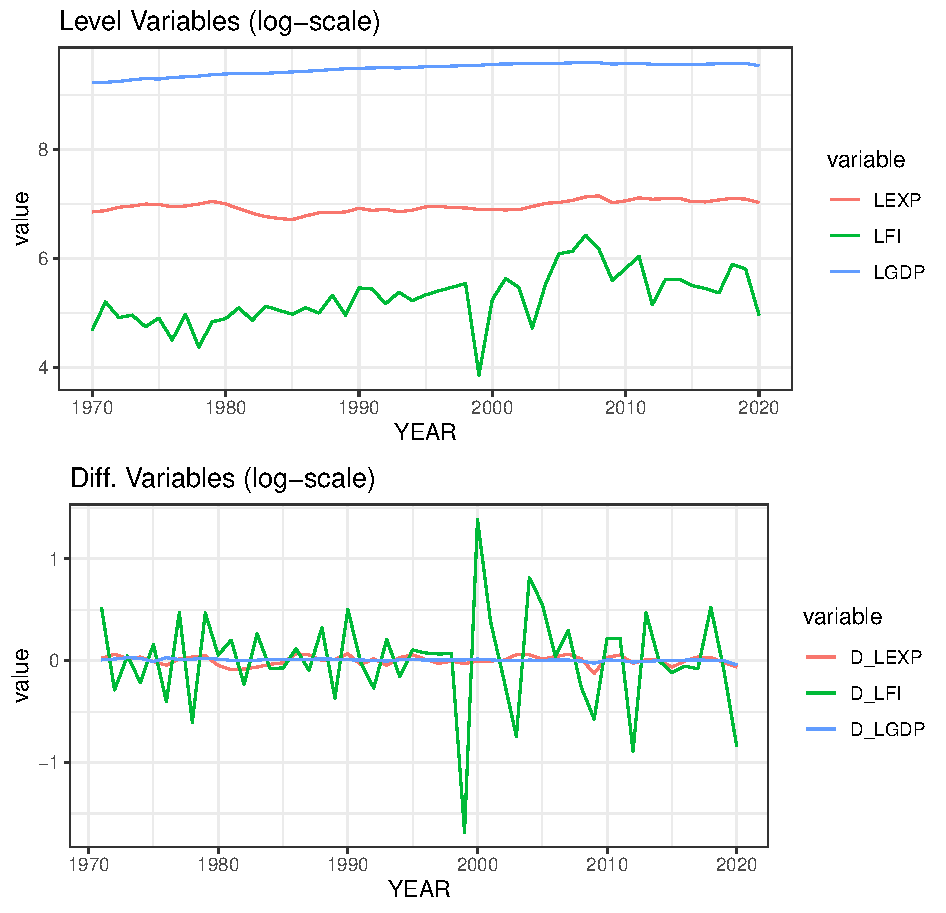
\includegraphics[scale=0.7]{figures/tsgraph2.pdf}
        \caption{log-GDP/export/investment graphs (level variables and first differences). Made with \CRANpkg{ggplot}.}
        \label{fig:plotemp2}
\end{figure}
\end{center}

\noindent Table \ref{tab:gdp1} shows the outcomes of the ADF test performed on each variable, which ensures that the integration order is not higher than one for all variables. Table \ref{tab:cointbig2} shows the results of bound and bootstrap tests performed in ARDL model by taking each variable, in turn, as the dependent one.
The following ARDL equations have been estimated:
\begin{enumerate}[I]
    \item First ARDL equation (GDP | EXP, FDI):
    \begin{align}
    \Delta \log \text{GDP}_{t}&=\alpha_{0.y} -
    a_{yy} \log \text{GDP}_{t-1} - {a}_{y.x_1}\log \text{EXP}_{t-1} - {a}_{y.x_2}\log \text{FDI}_{t-1} +\\\nonumber
    &\sum_{j=1}^{p-1}\gamma_{y.j} \Delta\log \text{GDP}_{t-j} +
    \sum_{j=1}^{s-1}\gamma_{x_1.j} \Delta\log \text{EXP}_{t-j} +
    \sum_{j=1}^{r-1}\gamma_{x_2.j} \Delta\log \text{FDI}_{t-j} +\\\nonumber
    &\omega_1 \Delta\log \text{EXP}_{t}+
    \omega_2 \Delta\log \text{FDI}_{t}+\nu_{t} 
    \end{align}.
    For this model, a degenerate case of the first type can be observed, while the simpler bound testing procedure does not signal cointegration.
    \item Second ARDL equation (EXP | GDP, FDI):
    \begin{align}
    \Delta \log \text{EXP}_{t}&=\alpha_{0.y} -
    a_{yy} \log \text{EXP}_{t-1} - {a}_{y.x_1}\log \text{GDP}_{t-1} - {a}_{y.x_2}\log \text{FDI}_{t-1} +\\\nonumber
    &\sum_{j=1}^{p-1}\gamma_{y.j} \Delta\log \text{EXP}_{t-j} +
    \sum_{j=1}^{s-1}\gamma_{x_1.j} \Delta\log \text{GDP}_{t-j} +
    \sum_{j=1}^{r-1}\gamma_{x_2.j} \Delta\log \text{FDI}_{t-j} +\\\nonumber
    &\omega_1 \Delta\log \text{GDP}_{t}+
    \omega_2 \Delta\log \text{FDI}_{t}+\nu_{t}. 
    \end{align}
  For this model, the ARDL bootstrap test indicates absence of cointegration, while the bound testing approach is inconclusive for the $F_{ind}$ test.
      \item Third ARDL equation (FDI | GDP, EXP):
    \begin{align}
    \Delta \log \text{FDI}_{t}&=\alpha_{0.y} -
    a_{yy} \log \text{FDI}_{t-1} - {a}_{y.x_1}\log \text{GDP}_{t-1} - {a}_{y.x_2}\log \text{EXP}_{t-1} +\\\nonumber
    &\sum_{j=1}^{p-1}\gamma_{y.j} \Delta\log \text{FDI}_{t-j} +
    \sum_{j=1}^{s-1}\gamma_{x_1.j} \Delta\log \text{GDP}_{t-j} +
    \sum_{j=1}^{r-1}\gamma_{x_2.j} \Delta\log \text{EXP}_{t-j} +\\\nonumber
    &\omega_1 \Delta\log \text{GDP}_{t}+
    \omega_2 \Delta\log \text{EXP}_{t}+\nu_{t}. 
    \end{align}
        For this model, the long-run cointegrating relationship is confirmed using both boostrap and bound testing. No spurious cointegration is detected.
\end{enumerate}
The code to load the data and perform the analysis (e.g. for Model I) is:
\begin{example}
    data("ita_macro")
    BCT_res_GDP = boot_ardl(data = ita_macro,
                         yvar = "LGDP",
                         xvar = c("LEXP", "LFI"),
                         maxlag = 5,
                         a.ardl = 0.1,
                         a.vecm = 0.1,
                         nboot = 2000,
                         case = 3,
                         a.boot.H0 = c(0.05),
                         print = T)
\end{example}
For the sake of simplicity, the conditional ARDL and VECM marginal models outputs included in each cointegrating analysis is omitted. The summary for the cointegration tests for Model I is called via
\begin{example}
    summary(BCT_res_GDP, out = "ARDL") # extract lags
    summary(BCT_res_GDP, out ="cointARDL") # ARDL cointegration
\end{example}
This empirical application further highlights the importance of dealing with inconclusive inference via the bootstrap procedure, while naturally including the effect of conditioning in the ARDL model, as highlighted in \citet{bertelli2022bootstrap}.
\begin{table}[htbp]
  \centering
  \resizebox{\textwidth}{!}{
    \begin{tabular}{lrrrrrrrrrrrr}
                 & \multicolumn{4}{c}{No Drift, No Trend} & \multicolumn{4}{c}{Drift, No Trend} & \multicolumn{4}{c}{Drift and Trend} \\
\cmidrule{2-13}   Variable & \multicolumn{1}{l}{Lag = 0} & \multicolumn{1}{l}{Lag = 1} & \multicolumn{1}{l}{Lag = 2} & \multicolumn{1}{l}{Lag = 3} & \multicolumn{1}{l}{Lag = 0} & \multicolumn{1}{l}{Lag = 1} & \multicolumn{1}{l}{Lag = 2} & \multicolumn{1}{l}{Lag = 3} & \multicolumn{1}{l}{Lag = 0} & \multicolumn{1}{l}{Lag = 1} & \multicolumn{1}{l}{Lag = 2} & \multicolumn{1}{l}{Lag = 3} \\
    \midrule$\log \text{GDP}_t$  & 0.99  & 0.974 & 0.941 & 0.796 & $<0.01$  & $<0.01$  & $<0.01$  & 0.084 & 0.99  & 0.99  & 0.99  & 0.99 \\
           $\log \text{FDI}_t$   & 0.572 & 0.599 & 0.675 & 0.725 & $<0.01$  & 0.0759 & 0.3199 & 0.5174 & $<0.01$  & 0.013 & 0.151 & 0.46 \\
           $\log \text{EXP}_t$  & 0.787 & 0.71  & 0.698 & 0.684 & 0.479 & 0.288 & 0.467 & 0.433 & 0.629 & 0.35  & 0.463 & 0.379 \\
\midrule       $\Delta\log \text{GDP}_t$ & $<0.01$  & $<0.01$64 & 0.0429 & 0.0402 & $<0.01$  & 0.0861 & 0.3989 & 0.4267 & $<0.01$  & $<0.01$  & 0.0166 & 0.017 \\
          $\Delta\log \text{FDI}_t$  & $<0.01$  & $<0.01$  & $<0.01$  & $<0.01$  & $<0.01$  & $<0.01$  & $<0.01$  & $<0.01$  & $<0.01$  & $<0.01$  & $<0.01$  & $<0.01$ \\
           $\Delta\log \text{EXP}_t$ & $<0.01$  & $<0.01$  & $<0.01$  & $<0.01$  & $<0.01$  & $<0.01$  & $<0.01$  & $<0.01$  & $<0.01$  & $<0.01$  & 0.0336 & 0.0315 \\
    \bottomrule
    \end{tabular}%
    }
  \caption{ADF preliminary test for the second example.}
  \label{tab:gdp1}%
\end{table}%
\begin{table}[htbp]
  \centering
  \resizebox{\textwidth}{!}{
    \begin{tabular}{ccc ccc ccc}
                 &       &       &  & \multicolumn{2}{c}{PSS / SMG Threshold} &  & \multicolumn{2}{c}{Outcome} \\
    \midrule
    \multicolumn{1}{c}{Model} & \multicolumn{1}{c}{Lags} & Test  &\multicolumn{1}{c}{Boot. Critical Values} &  \multicolumn{1}{c}{I(0) 5\%} & \multicolumn{1}{c}{I(1) 5\%} & Statistic &  \multicolumn{1}{c}{Boot} & \multicolumn{1}{c}{Bound} \\
    \midrule
\multirow{3}{*}{I} & \multirow{3}{*}{(1,1,0)} 
& $F_{ov}$  & 3.730 & 4.070 & 5.190 & 9.758 & \multirow{3}{*}{D1} & \multirow{3}{*}{N}\\
       &       
& $t$     & -2.020  & -2.860 & -3.530 & -2.338  &   &  \\
 &       
& $F_{ind}$ & 3.710  & 3.220 & 5.620 & 2.273                &       &  \\
\midrule
\multirow{3}{*}{II}       & \multirow{3}{*}{(1,0,0)} 
& $F_{ov}$  & 5.400  & 4.070 & 5.190 & 2.649  & \multirow{3}{*}{N}  & \multirow{3}{*}{U} \\        &       
& $t$     & -3.380 & -2.860 & -3.530 & -1.889  & &  \\ &       &       
 $F_{ind}$ & 5.630  & 3.220 & 5.620 & 3.481                &       &  \\

\midrule
\multirow{3}{*}{III} 
 & \multirow{3}{*}{(1,0,0)} 
& $F_{ov}$  & 5.360 & 4.070 & 5.190 & 6.716 & \multirow{3}{*}{Y} & \multirow{3}{*}{Y} \\
      &       
& $t$     & -3.550 & -2.860 & -3.530 & -4.202  &  &  \\&          
& $F_{ind}$ & 6.500 & 3.220 & 5.620 & 7.017          &       &  \\

    \bottomrule
    \end{tabular}%
    }
  \caption{Cointegration analysis for the three ARDL equations in the Italian macroeconomic data. The optimal number of ARDL lags in the short-run - in the form $(y,x_1,x_2)$, matching the model definition - bootstrap critical values, bound test thresholds and test statistics for each test are shown (case III).\\ The outcome columns draw conclusions on each type of model (bootstrap or bound): Y = cointegrated, N = not cointegrated, D1 = degenerate of type 1, D2 = degenerate of type 2, U = inconclusive inference.}
  \label{tab:cointbig2}%
\end{table}% 
\section{Conclusion}\label{sec:end}
The \CRANpkg{bootCT} package allows the user to perform bootstrap cointegration tests in ARDL models by overcoming the problem of inconclusive inference which is a well-known drawback of standard bound tests. 
The package makes use of different functions.
The function \code{boot\_ardl} performs the bootstrap tests, and it acts as a wrapper of both the bootstrap and the standard bound tests, including also the Johansen test on the independent variables of the model. Finally, it also performs the bound $F$-test on the lagged independent variables, so far not available in other extant \code{R} packages.
The function \code{sim\_vecm\_ardl}, which allows the simulation of multivariate time series data following a user-defined DGP, enriches the available procedures for multivariate data generation, while the function \code{lag\_mts} provides a supporting tool in building datasets of lagged variables for any practical purpose. Finally, the use of Rcpp functions gives a technical advantage in terms of computational speed, performing the bootstrap analysis within an acceptable time frame.

\newpage
\section{Appendix}\label{sec:appendix}
\subsection{Section A - the methodological framework of (conditional) VECM and ARDL models} \label{sec:appendixa}
Expanding the matrix polynomial $\mathbf{A}(z)$ about $z=1$, yields
\begin{equation}\label{eq:polyamat}
\mathbf{A}(z)=\mathbf{A}(1)z+(1-z)\boldsymbol{\Gamma}(z),
\end{equation}
where
\begin{equation}
\mathbf{A}(1)=\mathbf{I}_{K+1}-\sum_{j=1}^{p}\mathbf{A}_{j}
\end{equation}
\begin{equation}\label{eq:polygamma}
\boldsymbol{\Gamma}(z)=\mathbf{I}_{K+1}-\sum_{i=1}^{p-1}\boldsymbol{\Gamma}_{i}z^i, \enspace \enspace \boldsymbol{\Gamma}_{i}=-\sum_{j=i+1}^{p}\mathbf{A}_j.
\end{equation}
The VECM model \eqref{eq:vecm} follows accordingly, and
\begin{equation}\label{eq:vecmint}
\boldsymbol{\alpha}_0=\mathbf{A}(1)\boldsymbol{\mu}+(\boldsymbol{\Gamma}(1)-\mathbf{A}(1))\boldsymbol{\eta}, \enspace \enspace \enspace \boldsymbol{\alpha}_1=\mathbf{A}(1)\boldsymbol{\eta}.
\end{equation}
Assuming that $\mathbf{A}(1)$ is singular and that 
the variables $\mathbf{x}_{t}$ are cointegrated. This entails the following 
\begin{align}\label{eq:factt}
    \mathbf{A}(1)=&\begin{bmatrix}
\underset{(1,1)}{a_{yy}} & \underset{(1,K)}{\mathbf{a}_{yx}'} \\ \underset{(K,1)}{\mathbf{a}_{xy}} & \underset{(K,K)}{\mathbf{A}_{xx}}  
\end{bmatrix}=\underset{(K+1,r+1)}{\mathbf{B}}\underset{(r+1,K+1)}{\mathbf{C}'}=\begin{bmatrix}b_{yy} & \mathbf{b}_{yx}'\\  \mathbf{b}_{xy} & \mathbf{B}_{xx} \end{bmatrix}\begin{bmatrix}c_{yy} & \mathbf{c}_{yx}'\\  \mathbf{c}_{xy} & \mathbf{C}_{xx}'\end{bmatrix}= \nonumber\\
=&\begin{bmatrix}b_{yy}c_{yy}+\mathbf{b}_{yx}'\mathbf{c}_{xy} & b_{yy}\mathbf{c}_{yx}'+\mathbf{b}_{yx}'\mathbf{C}_{xx}'\\
\mathbf{b}_{xy}c_{yy}+\mathbf{B}_{xx}\mathbf{c}_{xy} & \mathbf{b}_{xy}\mathbf{c}_{yx}'+ \mathbf{A}_{xx} \end{bmatrix}, \enspace \enspace \enspace rk(\mathbf{A}(1))=rk(\mathbf{B})=rk(\mathbf{C}),
\end{align}
where $\mathbf{B}$ and $\mathbf{C}$ are full column rank matrices arising from the rank-factorization of $\mathbf{A}(1)=\mathbf{B}\mathbf{C}'$ with $\mathbf{C}$ matrix of the long-run relationships of the process    
and $\mathbf{B}_{xx}$, $\mathbf{C}_{xx}$ arising from the rank factorization of $\mathbf{A}_{xx}=\mathbf{B}_{xx}\mathbf{C}_{xx}'$, with $rk(\mathbf{A}_{xx})=rk(\mathbf{B}_{xx})=rk(\mathbf{C}_{xx})=r$ \footnote{ If the explanatory variables are stationary $\mathbf{A}_{xx}$ is non-singular ($rk(\mathbf{A}_{xx})=K$), while when they are integrated but without cointegrating relationship $\mathbf{A}_{xx}$ is a null matrix }. \\
By partitioning the vectors $\boldsymbol{\alpha}_{0}$, $\boldsymbol{\alpha}_{1}$, the matrix $\mathbf{A}(1)$ and the polynomial matrix $\boldsymbol{\Gamma}(L)$ conformably to $\mathbf{z}_{t}$, as follows
\begin{equation}\label{eq:alphapart}
\boldsymbol{\alpha}_0=\begin{bmatrix}
\underset{(1,1)}{\alpha_{0y}}  \\ \underset{(K,1)}{\boldsymbol{\alpha}_{0x}} 
\end{bmatrix}, \enspace \enspace \enspace \boldsymbol{\alpha}_1=\begin{bmatrix}
\underset{(1,1)}{\alpha_{1y}}  \\ \underset{(K,1)}{\boldsymbol{\alpha}_{1x} }
\end{bmatrix}
\end{equation}
\begin{equation}\label{eq:coeffpart}
\mathbf{A}(1)=\begin{bmatrix}
\underset{(1,K+1)}{\mathbf{a}'_{(y)}}  \\ \underset{(K,K+1)}{\mathbf{A}_{(x)}} 
\end{bmatrix}
=\begin{bmatrix}
\underset{(1,1)}{a_{yy}} & \underset{(1,K)}{\mathbf{a}'_{yx}}  \\ \underset{(K,1)}{\mathbf{a}_{xy}} & \underset{(K,K)}{\mathbf{A}_{xx} }
\end{bmatrix}, 
\enspace \enspace \enspace
\boldsymbol{\Gamma}(L)=\begin{bmatrix}
\underset{(1,K+1)}{\boldsymbol{\gamma}'_{y}(L)}  \\ \underset{(K,K+1)}{\boldsymbol{\Gamma}_{(x)}(L)} 
\end{bmatrix}
=\begin{bmatrix}
\underset{(1,1)}{\gamma_{yy}(L)} & \underset{(1,K)}{\boldsymbol{\gamma}'_{yx}(L)}  \\ \underset{(K,1)}{\boldsymbol{\gamma}_{xy}(L)} & \underset{(K,K)}{\boldsymbol{\Gamma}_{xx}(L) }
\end{bmatrix}
\end{equation},
and substituting \eqref{eq:epsilonx} into \eqref{eq:vecm} yields
\begin{equation}\label{eq:condsys}
\Delta\mathbf{z}_t=\begin{bmatrix}
\Delta y_{t} \\ \Delta\mathbf{x}_{t} 
\end{bmatrix}=\begin{bmatrix}
\alpha_{0.y} \\ \boldsymbol{\alpha}_{0x} 
\end{bmatrix} + \begin{bmatrix}
\alpha_{1.y} \\ \boldsymbol{\alpha}_{1x} 
\end{bmatrix}t- \begin{bmatrix}
\mathbf{a}'_{(y).x} \\ \mathbf{A}_{(x)} 
\end{bmatrix}\begin{bmatrix}
y_{t-1} \\ \mathbf{x}_{t-1} 
\end{bmatrix} + \begin{bmatrix}
\boldsymbol{\gamma}'_{y.x}(L) \\ \boldsymbol{\Gamma}_{(x)}(L) 
\end{bmatrix}\Delta\mathbf{z}_t+\begin{bmatrix}
\boldsymbol{\omega}'\Delta\mathbf{x}_{t} \\ \mathbf{0} 
\end{bmatrix}+\begin{bmatrix}
{\nu}_{yt} \\ \boldsymbol{\varepsilon}_{xt} 
\end{bmatrix} 
\end{equation},
where 
\begin{equation}\label{eq:condintt}
\alpha_{0.y}=\alpha_{0y}-\boldsymbol{\omega}'\boldsymbol{\alpha}_{0x}, \enspace \enspace \enspace \alpha_{1.y}=\alpha_{1y}-\boldsymbol{\omega}'\boldsymbol{\alpha}_{1x}
\end{equation}
\begin{equation}\label{eq:condAmat}
\mathbf{a}'_{(y).x}=\mathbf{a}'_{(y)}-\boldsymbol{\omega}'\mathbf{A}_{(x)}, \enspace \enspace \enspace \boldsymbol{\gamma}'_{y.x}(L)=\boldsymbol{\gamma}_{y}'(L)-\boldsymbol{\omega}'\boldsymbol{\Gamma}_{(x)}(L).
\end{equation}
According to \eqref{eq:condsys}, the long-run relationships of the VECM turn out to be now included in the matrix
\begin{equation}\label{eq:condAmat2}
\begin{bmatrix}
\mathbf{a}'_{(y).x} \\ \mathbf{A}_{(x)} 
\end{bmatrix}=\begin{bmatrix}
a_{yy}-\boldsymbol{\omega}'\mathbf{a}_{xy} & \mathbf{a}_{yx}'-\boldsymbol{\omega}'\mathbf{A}_{xx} \\ \mathbf{a}_{xy}&\mathbf{A}_{xx} 
\end{bmatrix}.
\end{equation}
To rule out the presence of long-run relationships between $y_{t}$ and $\mathbf{x}_{t}$ in the marginal model, 
the $\mathbf{x}_{t}$ variables are assumed to be exogenous with respect to the ARDL parameters, that is $\mathbf{a}_{xy}$ is assumed to be a null vector.
Accordingly, the long-run matrix in \eqref{eq:condAmat2} becomes
\begin{equation}\label{eq:cond}
\widetilde{\mathbf{A}}=\begin{bmatrix}a_{yy} & \mathbf{a}'_{yx}-\boldsymbol{\omega}'\mathbf{A}_{xx} \\ \mathbf{0} & \mathbf{A}_{xx} 
\end{bmatrix}=\begin{bmatrix}
a_{yy} & \widetilde{\mathbf{a}}_{y.x}' \\ \mathbf{0}&\mathbf{A}_{xx}\end{bmatrix} =\begin{bmatrix}
b_{yy}c_{yy} & b_{yy}\mathbf c_{yx}'+(\mathbf{b}_{yx}'-\boldsymbol{\omega}'\mathbf{B}_{xx})\mathbf{C}_{xx}' \\ \mathbf{0}& \mathbf{B}_{xx}\mathbf{C}_{xx}'\end{bmatrix}.
\end{equation}
After these algebraic transformations, the ARDL equation for $\Delta y_{t}$ can be rewritten as in \eqref{eq:ardl}.\\
In light of the factorization \eqref{eq:factt}
of the matrix $\mathbf{A}(1)$, the long-run equilibrium vector $\boldsymbol{\theta}$ can be expressed as
\begin{equation}\label{eq:thetat}
\boldsymbol{\theta}'=
-\frac{1}{a_{yy}}\underset{(1,r+1)}{\left[b_{yy}\enspace\enspace(\mathbf{b}_{yx}-\boldsymbol{\omega}'\mathbf{B}_{xx})\right]}
\underset{(r+1,K)}{\begin{bmatrix} \mathbf{c}'_{yx}\\ \mathbf{C}'_{xx} \end{bmatrix}},
\end{equation}
where $\widetilde{\mathbf{a}}_{y.x}=\mathbf{a}_{yx}-\boldsymbol{\omega}'\mathbf{A}_{xx}$.\\
Bearing in mind that $\mathbf{C}'_{xx}$ is the cointegrating matrix for the variables $\mathbf{x}_t$, the equation \eqref{eq:thetat} leads to the following conclusion
\begin{equation}\label{eq:rank}
rk\begin{bmatrix}\mathbf{c}'_{yx}\\ \mathbf{C}'_{xx}\end{bmatrix}=\begin{cases}
r  \to \enspace y_{t} \sim I(0) \\
r+1 \to \enspace y_{t} \sim I(1) 
\end{cases},
\end{equation}
where $r=rk(\mathbf{A}_{xx})$ and $0 \leq r\leq K$.  \\

\subsection{Section B - Intercept and trend specifications}\label{sec:appendixb}
 ~\citet{pesaran2001} introduced five different specifications for the ARDL model, which depend on the deterministic components that can be absent or restricted to the values they assume in the parent VAR model. In this connection, note that, in light of \eqref{eq:vecmint}, the drift and the trend coefficient in the conditional VECM \eqref{eq:condsys} are defined as
\begin{equation}
\boldsymbol{\alpha_{0}}^{c}=\widetilde{\mathbf{A}}(1)(\boldsymbol{\mu}-\boldsymbol{\eta})+\widetilde{\boldsymbol{\Gamma}}(1)\boldsymbol{\eta} , \enspace \enspace 
\boldsymbol{\alpha_{1}}^{c}=\widetilde{\mathbf{A}}(1)\boldsymbol{\eta}, 
\end{equation}
where $\widetilde{\mathbf{A}}(1)$ is as in \eqref{eq:cond} and $\widetilde{\boldsymbol{\Gamma}}(1)=\begin{bmatrix} \boldsymbol{\gamma}_{y.x}'(1) \\ \boldsymbol{\Gamma}_{(x)}(1) \end{bmatrix}$.\\
Accordingly, after partitioning the  mean and the drift vectors as 
\begin{equation}
\underset{(1,K+1)}{\boldsymbol{\mu}'}=[\underset{(1,1)}{\mu_{y}},\underset{(1,K)}{\boldsymbol{\mu}_x'}], \enspace \underset{(1,K+1)}{\boldsymbol{\eta}'}=[\underset{(1,1)}{\eta_{y}},\underset{(1,K)}{\boldsymbol{\eta}_{x}'}], 
\end{equation}
the intercept and the coefficient of the trend of the ARDL equation \eqref{eq:ardl} are defined as
\begin{equation}
\alpha_{0.y}^{EC}
= \mathbf{e}_{1}'\boldsymbol{\alpha_{0}}^{c}
=a_{yy}\mu_{y}-\widetilde{\mathbf{a}}'_{y.x}\boldsymbol{\mu}_{x}+\boldsymbol{\gamma}'_{y.x}(1)\boldsymbol{\eta}=a_{yy}(\mu_{y}-\boldsymbol{\theta}'\boldsymbol{\mu}_{x})+\boldsymbol{\gamma}'_{y.x}(1)\boldsymbol{\eta}, \enspace 
\boldsymbol{\theta}'=-\frac{\widetilde{\mathbf{a}}'_{y.x}}{a_{yy}}
\end{equation}
\begin{equation}
\enspace \enspace \alpha_{1.y}^{EC}=\mathbf{e}_{1}'\boldsymbol{\alpha_{1}}^{c}=
a_{yy}\eta_{y}-\widetilde{\mathbf{a}}'_{y.x}\boldsymbol{\eta}_{x}=a_{yy}(\eta_{y}-\boldsymbol{\theta'}\boldsymbol{\eta}_{x}),
\end{equation}
where $\mathbf{e}_{1}$ is the $K+1$ first elementary vector.\\
In the error correction term 
\begin{equation}
EC_{t-1}=y_{t-1}-\theta_{0}-\theta_{1}t-\boldsymbol{\theta}'\mathbf{x}_{t-1}
\end{equation}
the parameters that partake in the calculation of intercept and trend are
\begin{equation}
\theta_{0}=\mu_{y}-\boldsymbol{\theta}'\boldsymbol{\mu}_{x}, \enspace  \theta_{1}=\eta_{y}-\boldsymbol{\theta}'\boldsymbol{\eta}_{x}.
\end{equation}
In particular, these latter are not null only when they are assumed to be restricted in the model specification.\\
The five specifications proposed by ~\citet{pesaran2001} are
\begin{enumerate}[I]
\item \textit{No intercept and no trend}:
\begin{equation}
\boldsymbol{\mu}=\boldsymbol{\eta}=\mathbf{0}. 
\end{equation}
It follows that
\begin{equation}
\theta_{0}=\theta_{1}=\alpha_{0.y}=\alpha_{1.y}=0.
\end{equation}
Accordingly, the model is as in \eqref{eq:case1}.

\item \textit{Restricted intercept and no trend}:
\begin{equation}
\boldsymbol{\alpha}_{0}^{c}= \widetilde{\mathbf{A}}(1)\boldsymbol{\mu},\enspace \enspace  \boldsymbol{\eta}=\mathbf{0},
\end{equation}
which entails
\begin{equation}
\theta_0 \neq 0 \enspace\enspace\alpha_{0.y}^{EC}=a_{yy}\theta_{0}, \enspace \enspace
\alpha_{0.y}=\theta_{1}=\alpha_{1.y}=0.
\end{equation}
Therefore, the intercept stems from the EC term of the ARDL equation. The model is specified as in \eqref{eq:case2}

\item \textit{Unrestricted intercept and no trend}:
\begin{equation}
\boldsymbol{\alpha}_{0}^{c}\neq\widetilde{\mathbf{A}}(1)\boldsymbol{\mu}, \enspace \enspace \boldsymbol{\eta}=\mathbf{0}.
\end{equation}
Thus,
\begin{equation}
\alpha_{0.y}\neq 0,\enspace \enspace \theta_{0}=\theta_{1}=\alpha_{1.y}=0.
\end{equation}
Accordingly, the model is as in \eqref{eq:case3}.

\item \textit{Unrestricted intercept, restricted trend}:
\begin{equation}\boldsymbol{\alpha_{0}}^{c}\neq\widetilde{\mathbf{A}}(1)(\boldsymbol{\mu}-\boldsymbol{\eta})+\widetilde{\boldsymbol{\Gamma}}(1)\boldsymbol{\eta}\enspace \enspace {\boldsymbol{\alpha}}_{1}^{c}=\widetilde{\mathbf{A}}(1)\boldsymbol{\eta},
\end{equation}
which entails
\begin{equation}
\alpha_{0.y} \neq 0,\enspace \enspace 
\theta_{0}=0 \enspace \enspace
\theta_{1}\neq 0\enspace\enspace
\alpha_{1.y}^{EC}=a_{yy}\theta_1\enspace\enspace 
\alpha_{1.y}=0.
\end{equation}
Accordingly, the trend stems from the EC term of the ARDL equation. The model is as in \eqref{eq:case4}.
\item \textit{Unrestricted intercept, unrestricted trend}:
\begin{equation}
\boldsymbol{\alpha_{0}}^{c}\neq\widetilde{\mathbf{A}}(1)(\boldsymbol{\mu}-\boldsymbol{\eta})+\widetilde{\boldsymbol{\Gamma}}(1)\boldsymbol{\eta} \enspace \enspace {\boldsymbol{\alpha}}_{1}^{c}\neq\widetilde{\mathbf{A}}(1)\boldsymbol{\eta}.
\end{equation}
Accordingly,
\begin{equation} \alpha_{0.y} \neq 0 \enspace \enspace\alpha_{1.y} \neq 0, \enspace \enspace\theta_{0}=\theta_{1}=0.
\end{equation}
The model is as in \eqref{eq:case5}.
\end{enumerate}
\newpage



\bibliography{vacca-zoia-bertelli}

\address{Gianmarco Vacca\\
  Department of Economic Policy. Università Cattolica del Sacro Cuore\\
  Largo Gemelli, 1, Milan.\\
  Italy\\
  (0000-0002-8996-5524)\\
  \email{gianmarco.vacca@unicatt.it}}

\address{Maria Zoia\\
  Department of Economic Policy. Università Cattolica del Sacro Cuore\\
  Largo Gemelli, 1, Milan.\\
  Italy\\
  (0000-0002-8169-781X)\\
  \email{maria.zoia@unicatt.it}}
  
  \address{Stefano Bertelli\\
  CRO Area, Internal Validation and Controls Department, Operational Risk and ICAAP Internal Systems, 
  Intesa Sanpaolo, Milan\\
  Viale Stelvio, 55/57, Milan.\\
  Italy\\
  \email{stefano.bertelli@intesasanpaolo.com}}

